%
%--- 
%-----------------------------------
\chapter{ATOM-LIGHT INTERACTION}
\label{ch:atom-light-interaction}
%-----------------------------------
%--- 
%

In this chapter, we review several aspects of atom-light interaction \cite{weiner2003light} to properly approach the atomic dynamics in magneto-optical traps. First of all, we shall explore the basic concepts through \textbf{the phenomenological Einstein rate equations} \cite{foot2005atomic}, a "semi-quantum" model where atoms absorb and emit light at a defined rate. Afterwards, we invoke the quantum mechanics apparatus through the \textbf{density operator} and the \textbf{master equation} \cite{steck2007quantum} to analyze coherence effects and line broadening mechanisms. We thoroughly discuss the case of a two-level atom interacting with a monochromatic radiation through the semiclassical approach. Finally, we brief discuss conditions in which electric dipole transitions are allowed.


% Rate Equations Model
%-----------------------------------
%
%-----------------------------------
\section{Rate equations model}
\label{sec:rate-equations-model}
%-----------------------------------
%

A simple approach to introduce the essential aspects of atom-light interaction was proposed by Einstein in 1917. Although this theory does not take coherent effects into account, it is justified within the quantum mechanics framework in appropriate limits. Einstein assumed discrete energy levels for both atom and light. In this context, the electromagnetic radiation is composed of packets of energy $ \hbar \omega $ and momentum $ \hbar \omega / c $ known as photons, where $ \omega $ is the angular frequency, $ \hbar = h / 2\pi$ is the reduced Planck constant, and $ c $ is the speed of light. Einstein also postulated phenomenological rate equations to describe two-level atomic transitions due to the absorption and emission of photons. Let us consider a two-level transition where the energy difference between the upper and lower level is $ \hbar \omega_0 $, and an electromagnetic radiation with spectral energy density $ u(\omega) $. In Figure \ref{fig:optical-transitions}, we illustrated the three possible transitions involving absorption and emission of photons.

Let us consider a dilute atomic gas with number density $ n_1(t) $ of atoms in the lower level and number density $ n_2(t) $ of atoms in the upper level after a period of time $ t $. The Einstein rate equations express the time evolution of $ n_1 $ and $ n_2 $ so that
\begin{equation}
	\frac{d n_1}{dt} = - \frac{d n_2}{dt} = - B_{12} u(\omega_0) n_1 + B_{21} u(\omega_0) n_2 + A n_2,
	\label{eq:Einstein-rate-equations}
\end{equation}
where $ B_{12} u(\omega_0) $, $ B_{21} u(\omega_0) $, and $ A $ are phenomenological rates associated with the stimulated absorption, stimulated emission and spontaneous emission respectively. The rates associated with stimulated processes are proportional to the spectral density energy and therefore theses processes only happen in the presence of a light field. 

\begin{figure}[H]
	\caption{Optical two-level transitions}
	\begin{subfigure}[t]{0.32\textwidth}
		\centering
		\subcaption{\textbf{Stimulated absorption}}
		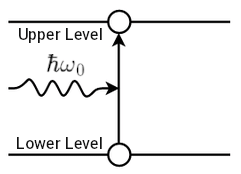
\includegraphics[width=0.8\textwidth]{USPSC-img/stimulated_absorption.png}
		\vspace{5pt}
		\legend{An atom in the lower level goes into the upper level absorbing a photon with energy $ \hbar \omega_0 $ from a light field with $ u(\omega_0) > 0 $.}
		\label{img:stimulated-absorption}
	\end{subfigure}
	\hfill
	\begin{subfigure}[t]{0.32\textwidth}
		\centering
		\subcaption{\textbf{Stimulated emission}}
		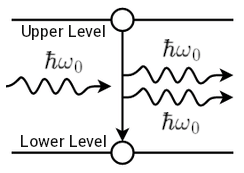
\includegraphics[width=0.8\textwidth]{USPSC-img/stimulated_emission.png}
		\vspace{5pt}
		\legend{An atom in the upper level decays into the lower level in the presence of a light field with $ u(\omega_0) > 0 $, emitting a photon with energy $\hbar \omega_0 $ similar to the photons in the light field.}
		\label{img:stimulated-emission}
	\end{subfigure}
	\hfill
	\begin{subfigure}[t]{0.32\textwidth}
		\centering
		\subcaption{\textbf{Spontaneous emission}}
		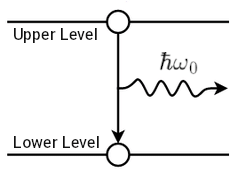
\includegraphics[width=0.8\textwidth]{USPSC-img/spontaneous_emission.png}
		\vspace{5pt}
		\legend{An atom in the upper level emits an isotropic photon with energy $ \hbar \omega_0 $ spontaneously, decaying into the lower level.}
		\label{img:spontaneous-emission}
	\end{subfigure}

	\legend{Source: Author}
	\vspace{-20pt}
	\label{fig:optical-transitions}
\end{figure}

%
%-----------------------------------
\subsection{Relation between the Einstein coefficients}
%-----------------------------------
%

A dilute atomic gas at temperature $ T $ in thermal equilibrium establishes a steady state in which $ n_1 $ and $ n_2 $ are constants of time ($ d_{t} n_1 = - d_{t} n_2 = 0 $). In this condition, from equation (\ref{eq:Einstein-rate-equations}), the spectral energy density is
\begin{equation}
	u({\omega_0}) = \frac{A}{(n_1 / n_2) B_{12} - B_{21}}.
	\label{eq:spectral-energy-thermal-equilibrium}
\end{equation}
Considering a fixed number of atoms $ n = n_1 + n_2 $, the system are represented by the canonical ensemble and then the ratio $ n_1 / n_2 $ is associated with the Boltzmann distribution so that
\begin{equation}
	\frac{n_1}{n_2} = \frac{g_1}{g_2} \exp\left\{-\frac{\hbar \omega_0}{k_B T}\right\},
	\label{eq:Boltzmann-distribution}
\end{equation}
where $ g_1 $ and $ g_2 $ are the degeneracies of the lower and upper level, respectively, and $ k_B $ is the Boltzmann constant. Einstein evaluated atoms in a region of black body radiation,  in which the spectral energy density of the light is consistent with the Planck distribution law given by
\begin{equation}
	u(\omega_0) = \frac{\hbar \omega_0^3}{\pi^2 c^3} \frac{1}{e^{\hbar \omega_0 / k_B T} - 1}.
	\label{eq:Planck-distribution}
\end{equation}
Comparing (\ref{eq:spectral-energy-thermal-equilibrium}), (\ref{eq:Boltzmann-distribution}), and (\ref{eq:Planck-distribution}), we obtain
\begin{equation} 
	B \equiv B_{21} = \frac{g_1}{g_2} B_{12}
	\label{eq:relation-B21-B12}
\end{equation}
and
\begin{equation} 
	A = \frac{\hbar \omega_0^3}{\pi^2 c^3} B.
	\label{eq:relation-A-B}
\end{equation}
The Einstein coefficients are properties of the atoms. Thereby the equations (\ref{eq:relation-A-B}) and (\ref{eq:relation-B21-B12}) are valid for any electromagnetic radiation, from narrow bandwidth radiation to broadband light. If we know one of the three rate coefficients, we can always determine the other two.

It is worthwhile to compare the spontaneous emission rate $ A $ to the stimulated emission rate $ B u(\omega_0) $ considering the equations (\ref{eq:Planck-distribution}) and (\ref{eq:relation-A-B}) so that
\begin{equation} 
	\frac{A}{B u(\omega_0)} = e^{\hbar \omega_0 / k_B T} - 1.
\end{equation}
Spontaneous emission dominates for high frequencies (visible, UV, X-ray), $ \hbar \omega_0 \gg k_B T $, but stimulated emission is more relevant for small frequencies (far IR, microwaves, radio waves).

%
%-----------------------------------
\subsection{Probabilistic analysis for single atoms}
\label{sec:rate-equations-analysis-single-atoms}
%-----------------------------------
%

Previously, we consider the effect of the Einstein equations on an atomic sample. In this section, we shall analyze the effect of those equations on a single atom through the probability $ P(t) $ of finding an atom in the upper level\footnote{Analogously, we can define the probability of finding an atom in the lower level.} after a period $t$,
\begin{equation}
	P(t) = \frac{n_2}{n_1 + n_2} = \frac{n_2(t)}{n}.
	\label{eq:probability-upper-level}
\end{equation}

From now on, for simplicity, we shall consider non-degenerate atomic transitions ($ g_1 = g_2 = 1 $). We also shall call the lower level as \textit{ground state} and the upper level as \textit{excited state}. The probability distribution $ \rho(t) $ of finding an atom in the excited state between the instants $t$ and $t + dt$ is given by
\begin{equation}
	\rho(t) = \frac{dP}{dt} = (1 - 2P) B u(\omega_0) - A P,
	\label{eq:distribution-upper-level}
\end{equation}
where we consider (\ref{eq:Einstein-rate-equations}), (\ref{eq:probability-upper-level}), and $ 1 - P = n_1 / n $.

Let us analyze a system only subject to spontaneous emission, assuming an atom in the absence of light ($ u(\omega) = 0 $) initially in the excited state ($ P(0) = 1 $). From (\ref{eq:distribution-upper-level}), we obtain
\begin{equation}
	P(t) = e^{-A t} \Rightarrow \rho(t) = A e^{-A t}
	\label{eq:probability-upper-level-spontenous-emission}
\end{equation}

The equation (\ref{eq:probability-upper-level-spontenous-emission}) indicates an exponential decay, which means an atom in the excited state certainly goes into the ground state after a long period ($ P(t) \longrightarrow 0 $). Therefore, we can interpret $ A $ as a \textit{relaxation rate}. The average time $ \tau $ in which an atom remains in the excited state, also known as \textit{lifetime}, is given by
\begin{equation}
	\tau = \int_{0}^{\infty} t \rho(t) dt = \int_{0}^{\infty} A t e^{-A t} dt = \frac{1}{A} \Rightarrow A = \frac{1}{\tau}.
\end{equation}

In contrast, we can analyze the effect of stimulated processes considering $ B u(\omega_0) \gg A $. Let us assume an atom initially in the ground state ($ P(0) = 0 $). From equation (\ref{eq:distribution-upper-level}), we obtain
\begin{equation} 
	P(t) = \frac{1 - e^{-\alpha t}}{2}
	\label{eq:probability-stimulated-processes}
\end{equation}
where $ \alpha \equiv 2 B u(\omega_0) $ is the rate in which the radiation raises (or "pumps") atoms into the excited state due to stimulated process, also known as \textit{pumping rate}. The equation (\ref{eq:probability-stimulated-processes}) shows that the strong driving of a transition leads to its \textit{saturation} ($ P(t) \longrightarrow 1/2 $). In other words, the atomic ensemble goes into complete transparency.

Finally, let us assume an atom initially in the ground state subjected to the effect of both stimulated and spontaneous processes. In this situation, the solution of (\ref{eq:distribution-upper-level}) is
\begin{equation}
	P(t) = \frac{1/2}{1 + A / \alpha}(1 - e^{-(A + \alpha)t})
	\label{eq:probability-upper-level-non-degenerate-levels}
\end{equation}
The equation (\ref{eq:probability-upper-level-non-degenerate-levels}) also indicates a saturation so that
\begin{equation}
	\lim_{t \rightarrow \infty} P(t) = \frac{1/2}{1 + A / \alpha}.
\end{equation}

In the limits $ A \gg \alpha $ and $ A \ll \alpha $, we obtain $ P(t) \longrightarrow 0 $ and $ P(t) \longrightarrow 1/2 $, respectively. These results are expected from the previous analysis.

%
%-----------------------------------
\subsection{Spectral broadening}
\label{sec:spectral-broadening}
%-----------------------------------
%

In the previous section, we assume that the emitted and absorbed photons have a single frequency $ \omega_0 $. In this case, the probability to absorb or emit a photon is a sharp line centered at $ \omega = \omega_0 $ as illustrated in figure \ref{fig:shap-spectral-line}. However, in real situations, atoms can absorb and emit photons in a range of frequencies due to \textbf{line-broadening mechanisms} (section \ref{sec:line-broadening-mechanisms}), which is illustrated in figure \ref{fig:broadened-spectral-line}. 

\begin{figure}[H]
	\caption{Spectral broadening}
	\begin{subfigure}[t]{0.45\textwidth}
		\centering
		\subcaption{Sharp spectral line}
		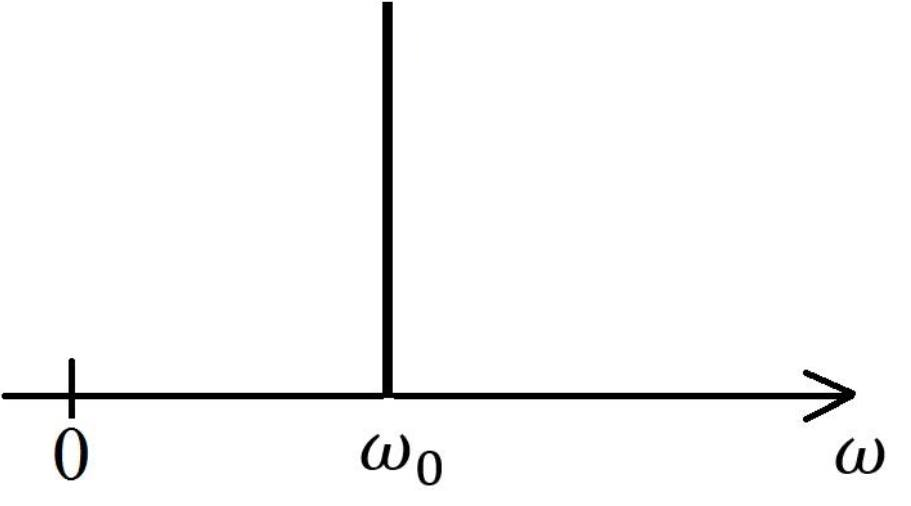
\includegraphics[width=0.8\textwidth]{USPSC-img/sharp_line.png}
		\vspace{5pt}
		\legend{Absorption or emission spectrum without line-broadening mechanisms so that we can assume the line shape $ g(\omega) = \delta(\omega - \omega_0) $.}
		\label{fig:shap-spectral-line}
	\end{subfigure}
	\hfill
	\begin{subfigure}[t]{0.45\textwidth}
		\centering
		\subcaption{Broadened spectral line}
		\vspace{8pt}
		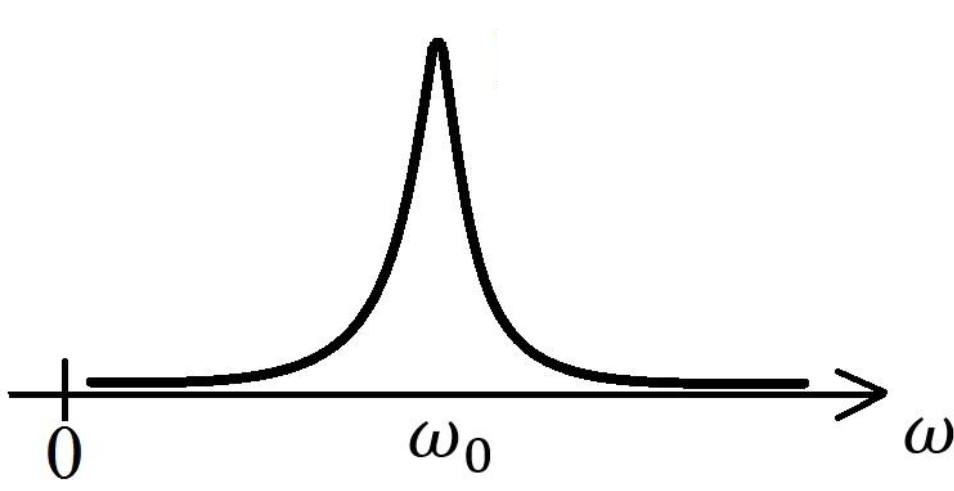
\includegraphics[width=0.8\textwidth]{USPSC-img/broadened_line.png}
		\vspace{5pt}
		\legend{Absorption or emission spectrum taking line-broadening mechanisms into account.}
		\label{fig:broadened-spectral-line}
	\end{subfigure}

	\legend{Source: \cite{valverde2016mecanismos}}
	\vspace{-20pt}
	\label{fig:spectral-broadening}
\end{figure}

We can take these mechanisms into account by introducing the normalized function $ g $ called \textbf{line shape function}. This function can be understood as the probability of absorbing or emitting a photon with frequency between $ \omega $ and $ \omega + d\omega $. A common $ g $ function in atomic spectroscopy is the \textit{Lorentzian}\footnote{Some authors define this distribution as a function of the frequency $ \nu $ instead of the angular frequency $ \omega = 2\pi\nu $.} (Cauchy distribution) given by
\begin{equation}
	g(\omega) = \frac{\Gamma'}{2\pi} \frac{1}{(\omega - \omega_0)^2 + (\Gamma' / 2)^2}\ \ \textrm{or}\ \ g(\Delta) = \frac{\Gamma'}{2\pi} \frac{1}{\Delta^2 + (\Gamma' / 2)^2},
\end{equation}
where $ \Delta = \omega - \omega_0 $ is the \textbf{detuning} and $ \Gamma' $ is the full width at half maximum (FWHM) also known as \textbf{spectral linewidth}. The main spectral linewidth is $ \Gamma' = A $, which is related to the energy-time uncertainty principle. Thus,
\begin{equation}
	g(\omega) = \frac{A}{2\pi} \frac{1}{(\omega - \omega_0)^2 + (A / 2)^2}\ \ \textrm{or}\ \ g(\Delta) = \frac{A}{2\pi} \frac{1}{\Delta^2 + (A / 2)^2}.
	\label{eq:line-shape-simplest-case}
\end{equation}

The probability distribution of finding an atom in the excited state taking the line shape function into account is given by
\begin{equation}
	\rho(t) = (1 - 2P) B \int_{0}^{\infty} u(\omega) g(\omega) d\omega - A P.
	\label{eq:distribution-upper-level-line-shape}
\end{equation}
For a broadband electromagnetic field, which means $ u(\omega) $ much broader than $ g(\omega) $, the equations (\ref{eq:distribution-upper-level-line-shape}) and (\ref{eq:distribution-upper-level}) are equivalent because
\begin{equation}
	\int_{0}^{\infty} u(\omega) g(\omega) d\omega \simeq u(\omega_0) \int_{0}^{\infty} g(\omega) d\omega = u(\omega_0).
	\label{eq:broadband-light-relation}
\end{equation}

%
%-----------------------------------
\subsection{Monochromatic light field}
%-----------------------------------
%

Let us consider a monochromatic electromagnetic field with frequency $ \omega $ interacting with an atom initially in the ground state. In the case, the spectral intensity $ I(\omega) $ and the spectral density energy $ u(\omega) $ of the light field is $ I(\omega') = c u(\omega') = I_0 \delta(\omega' - \omega) $, where $ I_0 $ is the total intensity and $ \delta(x) $ is the Dirac delta. Thus,
\begin{equation}
	\int_{0}^{\infty} u(\omega') g(\omega') d\omega' = \frac{I_0}{c} \int_{0}^{\infty} g(\omega') \delta(\omega' - \omega) d\omega' = \frac{I_0}{c} g(\omega).
	\label{eq:line-broadening-monochromatic-radiation}
\end{equation}
From equation (\ref{eq:distribution-upper-level-line-shape}) and (\ref{eq:line-broadening-monochromatic-radiation}), we obtain
\begin{equation}
	\rho(t) = (1 - 2P) \frac{\alpha(\omega)}{2} - A P,
	\label{eq:distribution-excited-state-monochromatic-light}
\end{equation}
where $ \alpha(\omega) = 2B(I_0 / c)g(\omega) $ is the \textbf{pumping rate}. The stationary solution of (\ref{eq:distribution-excited-state-monochromatic-light}) is given by
\begin{equation}
	P(t) = \frac{1 / 2}{1 + A / \alpha(\omega)} = \frac{1}{2} \frac{s(\omega)}{1 + s(\omega)},
	\label{eq:probability-excited-state-monochromatic-light}
\end{equation}
where $ s(\omega) = \alpha(\omega) / A $ is the \textbf{saturation parameter}, which defines the balance between pumping and relaxation. From equation (\ref{eq:relation-A-B}), we have
\begin{equation}
	s(\omega) = \frac{2\pi^2 c^2}{\hbar \omega_0^3} I_0 g(\omega) = \frac{2\lambda_0^3}{h c} I_0 g(\omega) = \frac{I_0}{I_s} \frac{g(\omega)}{g(\omega_0)},\ \ \textrm{where}\ \ I_s \equiv \frac{\hbar \omega_0^3}{2\pi^2 c^2 g(\omega_0)} .
	\label{eq:saturation-parameter-ERE}
\end{equation}
The intensity $ I_s $ is called \textbf{saturation intensity}. When $ s(\omega) \gg 1 $, stimulated processes are more significant than spontaneous emission, implying the saturation $ P \longrightarrow 1/2 $. When $ s(\omega) \ll 1 $, relaxation processes are predominant. In this case, the atom will certainly decay to the ground state, $ P \longrightarrow 0 $.

%
%-----------------------------------
\subsection{Absorption cross section}
\label{sec:absorption-cross-section}
%-----------------------------------
%

\begin{wrapfigure}{l}{0.45\textwidth}
	\centering
	\caption{Absorption Cross Section}
	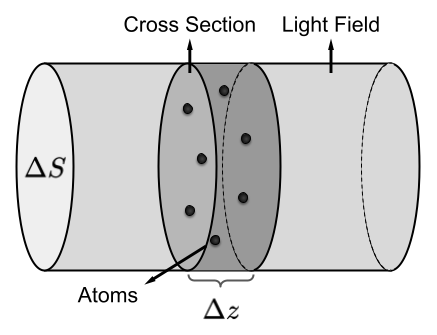
\includegraphics[width=0.43\textwidth]{USPSC-img/cross_section_scheme.png}
	\legend{Dilute atomic gas interacting with a electromagnetic radiation in a slab of thickness $ \Delta z $ and volume $ \Delta S \Delta z $. \\ Source: Author}
	\vspace{-15pt}
	\label{fig:absorption-cross-section}
\end{wrapfigure}

In atomic spectroscopic, it is common to analyze the attenuated or amplified light beam which passes through an atomic medium \cite{reinaudi2007strong, smith2011absorption, shu2004absorption}. Let us consider an electromagnetic beam with total spectral intensity $ I(\omega, z) $ propagating in the z-direction. This radiation passes through an atomic ensemble with $ n_1 $ atoms per volume in the ground state and $ n_2 $ atoms per volume in the excited state (figure \ref{fig:absorption-cross-section}), being attenuated or amplified in each slab of thickness $ \Delta z $ due to stimulated absorption. Its spectral intensity will be reduced by a fraction of $ n_1 \sigma(\omega) \Delta z $, where $ \sigma(\omega) $, known as \textbf{absorption cross-section}\footnote{The absorption cross-section is expressed in units of area}, is related to the probability that an atom will absorb an photon with angular frequency between $ \omega $ and $ \omega + d\omega $ from the light field on the section where this light passes on. Therefore, the lost spectral intensity is given $ \Delta I / I = - N \sigma \Delta z $ and then
\begin{equation}
	\frac{dI}{dz}(\omega, z) = - n_1 \sigma(\omega) I(\omega, z).
	\label{eq:lost-spectral-intensity}
\end{equation}
Besides the light attenuation due to stimulated absorption, there are also gain due to stimulated emission. Spontaneous emission does not contribute to the gain since the emitted light is isotropic. In this case, the light field will be amplified in each slab, increasing its intensity by a fraction of $ n_2 \sigma(\omega) \Delta z $. Here, the quantity $ \sigma $ gives the probability of emitting light stimulately. The absorption cross-section and the emission cross-section are the same since the absorption rate equals the emission rate ($ B_{12} = B_{21} $ when $ g_1 = g_2 $). Therefore, the light gain is given by
\begin{equation}
	\frac{dI}{dz}(\omega, z) = n_2 \sigma(\omega) I(\omega, z).
	\label{eq:spectral-density-power}
\end{equation}
From equations (\ref{eq:lost-spectral-intensity}) and (\ref{eq:spectral-density-power}), we obtain
\begin{equation}
	\frac{dI}{dz}(\omega, z) = - (n_1 - n_2) \sigma(\omega) I(\omega, z)
	\label{eq:net-spectral-density-power}
\end{equation}
where $ (dI / dz) \Delta S \Delta z $ is equivalent to the net spectral power (power per unit of frequency) gained or lost by the radiation in a slab of thickness $ \Delta z $ due to stimulated processes\footnote{Spontaneous emitted light does not come back to the radiation field, since it is isotropic.}. It is convenient to define a \textbf{net absorption cross-section} as 
\begin{equation}
	\sigma_{abs}(\omega) = \frac{n_1 - n_2}{n} \sigma(\omega) = (1 - 2P)\sigma(\omega),
	\label{eq:net-absorption-cross-section}
\end{equation}
where $ n = n_1 + n_2 $ is the total density number and $ P $ is the probability of finding an atom in the excited state. This cross-section is associated with the probability of an atom attenuating or amplifying an incident light due to stimulated processes. Solving the differential equation (\ref{eq:net-spectral-density-power}), we obtain
\begin{equation}
	I(\omega, z) = e^{-n\sigma_{abs}(\omega)t}I(\omega, 0),
	\label{eq:Beer-Lambert-law}
\end{equation}
In the regime of weak excitation such that $ n_2 \ll n_1 $, the total number density is approximately the number density of the atoms in the ground state $ n \simeq n_1 $ and then $ \sigma_{abs}(\omega) \simeq \sigma(\omega) $.

Let us assume a \textit{monochromatic} radiation whose frequency is $ \omega $ such that $  I(\omega', z) = I_0(z) \delta(\omega' - \omega) $ and $ u(\omega', z) = I(\omega', z) / c $. In this case, integrating equation (\ref{eq:net-spectral-density-power}) over all frequencies, we obtain the total power per unit of volume gained or lost by the radiation
\begin{equation}
	\frac{d I_0}{dz}(z) = -n\sigma_{abs}(\omega)I_0(z)\ \ \Rightarrow\ \ I_0(z) = I_0(0) e^{- n\sigma_{abs}(\omega)z}.
	\label{eq:Beer-Lambert-law-total-power}
\end{equation}
In the steady state, $ (dI_0/dz) $ equals the total power per unit of volume lost by spontaneous emission. Then, from equation (\ref{eq:Beer-Lambert-law-total-power}), we have
\begin{gather}
	n\sigma_{abs}(\omega) I_0 = A n_2 \hbar \int_0^{\infty} \omega g(\omega)d\omega.
	\label{eq:cross-section-expression}
\end{gather}
Since $ \omega_0 $ is much greater than the FWHM of $ g(\omega) $\footnote{The line shape function must be normalized over $ 0 $ to $ \infty $, which demands that the peak frequency $ \omega_0 $ of $ g(\omega) $ must be much greater than its FWHM.}, thus
\begin{equation}
	\int_0^{\infty} \omega g(\omega)d\omega \simeq \omega_0.
\end{equation}
Then, from equation (\ref{eq:cross-section-expression}), we have
\begin{equation}
	n \sigma_{abs}(\omega) I_0 = A n_2 \hbar \omega_0\ \Rightarrow\ \sigma_{abs}(\omega) = \frac{\hbar \omega_0}{I_0} A P,
	\label{eq:net-absorption-cross-section}
\end{equation}
where $ P = n_2 / n $. Therefore, in the steady state, the \textit{net absorption cross-section} can be understood as an area on which the photon flux of the incident beam passes through times the rate $ \Gamma P $ at which an atom scatters photons by spontaneous emission, i.e. the decay rate $ \Gamma $ times the probability of finding an atom in the excited state. From equations (\ref{eq:probability-excited-state-monochromatic-light}), (\ref{eq:saturation-parameter-ERE}), and (\ref{eq:net-absorption-cross-section}), we obtain
\begin{gather}
	\sigma(\omega) = \frac{\hbar \omega_0}{I_0} \frac{A}{2} s(\omega) = \overbrace{\frac{\hbar \omega_0}{I_s} \frac{A}{2}}^{\sigma_0} \frac{g(\omega)}{g(\omega_0)} = \sigma_0 \frac{g(\omega)}{g(\omega_0)}\ \ \textrm{and}
	\label{eq:absorption-cross-section-2}
	\\
	\sigma_{abs}(\omega) = \frac{\hbar \omega_0}{I_0} \frac{A}{2} \frac{s(\omega)}{1 + s(\omega)} = \sigma(\omega) \frac{1}{1 + s(\omega)},
	\label{eq:net-absorption-cross-section-2}
\end{gather}
where $ \sigma_0 \equiv \sigma(\omega_0) $ is the \textit{resonant absorption cross-section} which only depends on the properties of the atom ($ I_s$, $ \omega_0 $, and $ A $).




%-----------------------------------
%


% Two-level atom interaction with classical field
%-----------------------------------
%
%--- 
%-----------------------------------
\section{Two-level atom interacting with classical light field}
\label{sec:two-level-atom}
%-----------------------------------
%--- 
%

In the previous section, we consider phenomenological rate equations to study two-level atomic transitions. This approach does not contemplate coherence effects nor a fundamental understanding of line broadening mechanisms. In a first attempt, we can take the coherence effects into account assuming the interaction between a classical light field (electromagnetic waves) and an atom whose internal states are described by a quantum state vector $ \ket{\psi} $. Indeed, this is a proper treatment as long as we are only interested in stimulated processes. However, spontaneous emission comes from the interaction between atom and the vacuum modes of the quantized electromagnetic field, an incoherent relaxation process. Therefore, a single state vector is not sufficient to analyze an atom under both stimulated and spontaneous processes since such system is under decoherence. A proper description comes through the density operator (appendix \ref{ap:density-operator}), which describes a statistical mixture of quantum states. This approach allows us to study the system time evolution taking both coherent and incoherent processes into account through a master equation.

%
%-----------------------------------
\subsection{Two-level system and the Bloch sphere}
\label{sec:two-level-system-Bloch-sphere}
%-----------------------------------
%

Let us consider a system composed of only two quantum states $ \ket{1} $ and $ \ket{2} $, in which $ \ket{1} $ is the \textit{ground state} and $ \ket{2} $ is the excited state. An arbitrary two-dimensional density operator can be represent as
\begin{equation}
	\hat{\rho} = \left[ \begin{matrix} \rho_{1, 1} & \rho_{1, 2} \\ \rho_{2, 1} & \rho_{2, 2}\end{matrix}\right],
	\label{eq:density-operator-two-level-system}
\end{equation}
where $ \rho_{i,j} = \braket{i|\hat{\rho}|j} $. The diagonal terms represent probabilities so that $ \rho_{1,1} + \rho_{2,2} = 1 $, being $\rho_{1,1} $ and $ \rho_{2,2} $ real values. Also, $ \hat{\rho} $ must be hermitian and therefore $ \rho_{1,2} = (\rho_{2,1})^* $. The density matrix (\ref{eq:density-operator-two-level-system}) is represented on the basis
\begin{equation}
	\left\{\left[ \begin{matrix} 1 & 0 \\ 0 & 0 \end{matrix} \right],\ \left[ \begin{matrix} 0 & 1 \\ 0 & 0 \end{matrix} \right],\ \left[ \begin{matrix} 0 & 0 \\ 1 & 0 \end{matrix} \right],\ \left[ \begin{matrix} 0 & 0 \\ 0 & 1 \end{matrix} \right] \right\}.
\end{equation}
Another convenient basis is the \textbf{Pauli matrices basis},
\begin{equation}
	\left\{\sigma_x = \left[ \begin{matrix} 0 & 1 \\ 1 & 0 \end{matrix} \right],\ \sigma_y = \left[ \begin{matrix} 0 & -i \\ i & 0 \end{matrix} \right],\ \sigma_z = \left[ \begin{matrix} 1 & 0 \\ 0 & -1 \end{matrix} \right],\ \mathbb{I}_2 = \left[ \begin{matrix} 1 & 0 \\ 0 & 1 \end{matrix} \right] \right\},
\end{equation}
where $ \sigma_x $, $ \sigma_y $, and $ \sigma_z $ are the \textit{Pauli matrices}. An arbitrary density matrix on this basis is written as\footnote{For an arbitrary operator, we should have four coefficients $ [\hat{A}] = a_0 \mathbb{I} + a_1 \sigma_x + a_2 \sigma_y + a_3 \sigma_z $. In the case of the density matrix, we must have $ a_0 = 1/2 $ due to the property $ \Tr[\hat{\rho}] = 1 $.}
\begin{gather}
	\hat{\rho} = \frac{1}{2}(\mathbb{I}_2 + \mathbf{a} \cdot \vec{\sigma}) = \frac{1}{2}\left[ \begin{matrix} 1 + a_3 & a_1 - ia_2 \\ a_1 + i a_2 & 1 - a_3 \end{matrix} \right], 
	\label{eq:density-matrix-on-Pauli-basis}
	\\
	\textrm{where}\ \ \vec{\sigma} = \left[ \begin{matrix} \sigma_x \\ \sigma_y \\ \sigma_z \end{matrix} \right]\ \ \textrm{and}\ \ \mathbf{a} = \left[ \begin{matrix} a_1 \\ a_2 \\ a_3 \end{matrix} \right] \textrm{(\textbf{Bloch vector})}.
	\label{eq:Bloch-vector}
\end{gather}
In this representation, its eigenvalues are $ (1 \pm |\mathbf{a}|)/2$. Since they are probabilities, we must have $ 0 \leq (1 \pm |\mathbf{a}|)/2 \leq 1 \Rightarrow |\mathbf{a}| \leq 1 $. For the same reason, the diagonal terms, and then $ a_3 $, must be positive values. Furthermore, $ \hat{\rho} = \hat{\rho}^{\dagger} $, which implies $ a_1 = a_1^* $ and $ a_2 = a_2^* $. Hence, $ \mathbf{a} $ is a real vector. Comparing with the density matrix (\ref{eq:density-operator-two-level-system}), we have $ a_3 = \rho_{1,1} - \rho_{2,2} = p $ and $ (a_1 + i a_2) / 2 = \rho_{2,1} = q $, where $ p $ is known as \textbf{population inversion} and $ q $ is the \textit{coherence}. Then, the Bloch vector and the density matrix can be written as
\begin{equation}
	\mathbf{a} = \left[ \begin{matrix} 2\Re[q] \\ 2\Im[q] \\ p \end{matrix} \right] = \left[ \begin{matrix} q + q^* \\ i(q^* - q) \\ p \end{matrix} \right]\ \ \textrm{and}\ \ \hat{\rho} = \left[ \begin{matrix} (1 + p)/2 & q^{*} \\ q & (1 - p)/2 \end{matrix} \right].
	\label{eq:density-matrix-two-level-system}
\end{equation}
Taking the property $ |\mathbf{a}| \leq 1 $ into account, we can represent the Bloch vector in a ball of unitary radius known as \textbf{Bloch sphere} (although it is a ball, not a sphere) illustrated in figure \ref{fig:Bloch-sphere}. The axes are given by $x = 2\Re[q]$, $ y = 2\Im[q] $, and $ z = p $. When $ \hat{\rho} $ represent a pure state, we have
\begin{equation}
	\Tr[\hat{\rho}^2] = 1 \Rightarrow \frac{1}{2}(1 + |\mathbf{a}|^2) = 1 \Rightarrow |\mathbf{a}|^2 = 1.
\end{equation}
Therefore, the surface of the Bloch sphere represents all the pure states, whereas the inside corresponds to all the mixed states.

\noindent
\begin{minipage}{\textwidth}
	\begin{wrapfigure}{l}{0.45\textwidth}
		\centering
		\vspace{-10pt}
		\caption{Bloch sphere.}
		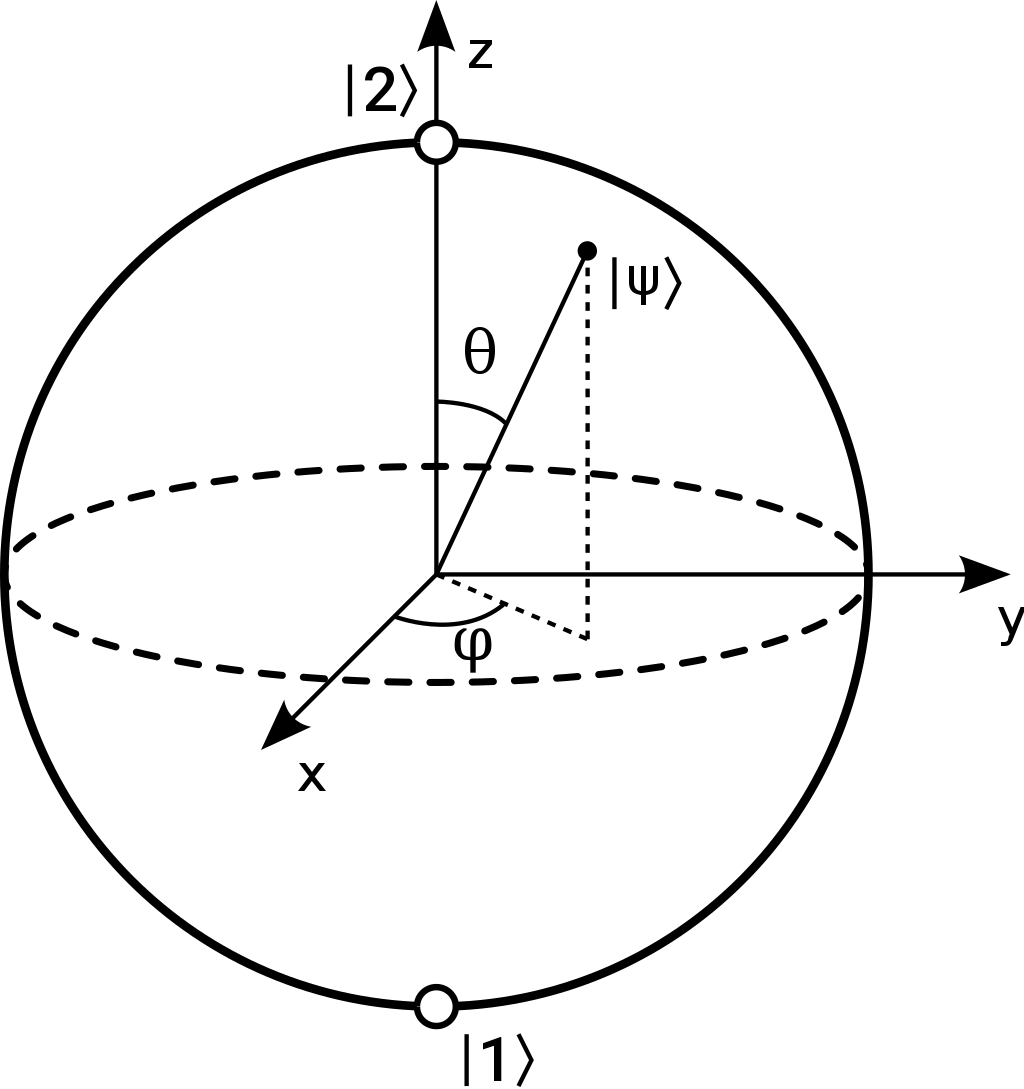
\includegraphics[width=0.35\textwidth]{USPSC-img/Bloch_sphere.png}
		\legend{Bloch sphere for a pure state given by \\ $ \ket{\psi} = \sin(\theta/2) \ket{1} + e^{i\phi} \cos(\theta/2) \ket{2} $. \\ Source: Author}
		\label{fig:Bloch-sphere}
		\vspace{-5pt}
	\end{wrapfigure}
	Let us consider a pure state $ \ket{\psi} = c_1\ket{1} + c_2\ket{2} $. Since a global phase is not measurable, we can assume $ \ket{\psi} = c_1 \ket{1} + c_2 e^{i\phi} \ket{2} $ where $ \phi $ is the phase difference between $ \ket{1} $ and $ \ket{2} $, and both $ c_1 $ and $ c_2 $ are real values. Moreover, $ c_1^2 + c_2^2 = 1 $, which allows us to associate $ c_1 $ and $ c_2 $ with a unique value $ \theta $ considering $ c_1 = \sin{(\theta/2)} $ and $ c_2 = \cos{(\theta/2)} $. Even though the value of $ \theta $ is not unique to represent $ c_1 $ and $ c_2 $, the point $ (\theta, \phi) $ is unique to represent $ \ket{\psi} $. Thus, a density operator $ \hat{\rho} = \ketbra{\psi}{\psi} $ of a pure state can be written as
	\begin{align}
		\hat{\rho} &= \sin^2(\theta/2) \ketbra{1}{1} + \cos^2(\theta/2) \ketbra{2}{2} + \nonumber 
		\\
		&+ \frac{1}{2}e^{-i\phi}\sin\theta \ketbra{1}{2} + \frac{1}{2}e^{i\phi}\sin\theta \ketbra{2}{1},
	\end{align}
\end{minipage}

\begin{equation}
	\hat{\rho} = \left[ \begin{matrix} \sin^2(\theta/2) & \frac{1}{2}e^{-i\phi}\sin\theta \\ \frac{1}{2}e^{i\phi}\sin\theta & \cos^2(\theta/2) \end{matrix} \right].
	\label{eq:density-matrix-pure-state-spherical-coordinates}
\end{equation}
From equations (\ref{eq:density-matrix-on-Pauli-basis}) and (\ref{eq:density-matrix-pure-state-spherical-coordinates}), we obtain the following Bloch vector
\begin{equation}
	\mathbf{a} = (\cos\phi \sin\theta, \sin\phi \sin\theta, \cos\theta),
\end{equation}
in which $ (\phi, \theta) $ are \textit{spherical coordinates} represented in figure \ref{fig:Bloch-sphere}.

%
%-----------------------------------
\subsection{Interaction Hamiltonian}
\label{sec:interaction-Hamiltonian}
%-----------------------------------

Let us consider a system formed by only two electronic states $ \{\ket{1}, \ket{2}\} $\footnote{Actually, there are many electronic states which can be relevant. However, in many cases, only two states are enough to described the interaction.}, each one is a possible state of a valence electron in an atom. This system is well described by the density operator $ \hat{\rho} $ given by (\ref{eq:density-matrix-two-level-system}). The dynamics of theses states in the absence of a light field is given by the following Hamiltonian
\begin{equation}
	 \hat{H}_0 = \hbar \omega_1 \ketbra{1}{1} + \hbar \omega_2 \ketbra{2}{2} = \hbar \omega_1 \hat{\sigma} \hat{\sigma}^{\dagger} + \hbar \omega_2 \hat{\sigma} \hat{\sigma}^{\dagger},
\end{equation}
where $ \hat{\sigma} \equiv \ketbra{1}{2} $ and $ \omega_1 < \omega_2 $. The lowest energy state $ \ket{1} $ is called \textit{ground state}, whereas the highest energy state $ \ket{2} $ is called \textit{excited state}. Since we are only concern with energy differences, we can shift the zero of energy adding $ - \hbar \omega_1 $ to each energy level so that
\begin{equation}
	\hat{H}_0 = \hbar \omega_0 \hat{\sigma}^{\dagger} \hat{\sigma} = \left[ \begin{matrix} 0 & 0 \\ 0 & \hbar \omega_0 \end{matrix} \right],
	\label{eq:atom-hamiltonian}
\end{equation}
where $ \omega_0 = \omega_2 - \omega_1 $ is the \textbf{resonant frequency}. The matrix in the equation (\ref{eq:atom-hamiltonian}) and also further matrix are represented on the basis $ \{\ket{1}, \ket{2}\} $. Moreover, we shall assume a monochromatic radiation whose \textit{electric field} $ \mathbf{E} $ is given by
\begin{equation}
	\mathbf{E}(\mathbf{r}, t) = \frac{\vec{\epsilon}}{2}(E_0 e^{i \mathbf{k} \cdot \mathbf{r} - i \omega t} + E_0^* e^{-(i \mathbf{k} \cdot \mathbf{r} - i \omega t)}),
	\label{eq:monochromatic-radiation}
\end{equation}
where $ \vec{\epsilon} = (\vec{\epsilon})^* $ is the \textit{polarization vector}, $ E_0 $ is the \textit{complex amplitude}, $ \mathbf{k} $ is the \textit{wave vector}, $ \omega $ is the \textit{angular frequency}, and $ \mathbf{r} $ is the \textit{position vector}. The interaction between the electric field $ \mathbf{E} $ and the \textit{electric dipole} formed by the valence electron and the atomic nucleus is the major atom-light interaction described by the following Hamiltonian
\begin{equation}
	\hat{V} = - \mathbf{d} \cdot \mathbf{E},
	\label{eq:dipole-interaction}
\end{equation}
where $ \mathbf{d} = - e \mathbf{r}_e  $ is the \textbf{dipole operator}, $ e \simeq 1.6 \times 10^{-19}C $ is the elementary charge, and $ \mathbf{r}_e $ is the valence electron position in the nucleus frame. The typical values of $ |\vec{\mu}| $ are around $ ea_B $\footnote{The \textit{debye} (symbol $ D $) is a standard unit measure for electric dipole moment in the atomic and molecular scale, $ 1 D \equiv 10^{-18} statC \cdot cm $. Historically, the debye was defined as the dipole moment of a system composed of two electric charges of opposite sign and equal magnitude $ 10^{-10} statC \simeq 0.2083 e $ separated by $ 1 \textrm{\AA} $.}, where $ a_B = 0.529 \textrm{\AA} = 0.529 \cdot 10^{-10}m $ is the \textit{Bohr radius}. Atoms do not have permanent dipole moment due to the parity of the electrons position. Hence, the dipole operator can be written as\footnote{We are assuming $ \braket{1|\mathbf{d}|1} = \braket{2|\mathbf{d}|2} = 0 $.}
\begin{gather}
	\mathbf{d} = (\vec{\mu})^* \hat{\sigma} + \vec{\mu} \hat{\sigma}^{\dagger},
	\label{eq:transition-dipole-moment}
\end{gather}
where $ \vec{\mu} \equiv \braket{2|\mathbf{d}|1} $ is the \textbf{transition dipole moment}. When $ |\vec{\mu}| = 0 $, the transition is said to be \textbf{dipole forbidden}. Then, from equations (\ref{eq:monochromatic-radiation}), (\ref{eq:transition-dipole-moment}), and (\ref{eq:dipole-interaction}), we obtain the following interaction Hamiltonian
\begin{gather}
	\hat{V}(t) = \frac{\hbar}{2} [(\tilde{\Omega}^*(\mathbf{r}) e^{- i \omega t} + \Omega^{*}(\mathbf{r})e^{i \omega t})\hat{\sigma} + (\Omega(\mathbf{r}) e^{- i \omega t} + \tilde{\Omega}(\mathbf{r})e^{i \omega t})\hat{\sigma}^{\dagger}],
	\label{eq:full-interaction-Hamiltonian}
	\\
	\Omega(\mathbf{r}) \equiv -\frac{E_0(\vec{\epsilon} \cdot \vec{\mu})}{\hbar}e^{i\mathbf{k}\cdot\mathbf{r}}\ \textrm{and}\ \tilde{\Omega}(\mathbf{r}) \equiv -\frac{E_0^* (\vec{\epsilon} \cdot \vec{\mu})}{\hbar}e^{-i\mathbf{k}\cdot\mathbf{r}},
	\label{eq:Rabi-frequency}
\end{gather}
where $ \Omega(\mathbf{r}) $ and $ \tilde{\Omega}(\mathbf{r}) $ are known as \textbf{Rabi frequencies}\footnote{Both $ \Omega $ and $ \tilde{\Omega} $ have the same amplitude $ |\Omega| = |\tilde{\Omega}| $ but different phases.}.

The minimum wavelength of non-ionizing radiation, which is the typical spectral range in laser cooling experiments, is around $100 nm = 1000 \textrm{\AA} $, whereas the atomic size is around the Bohr radius $ a_B \simeq 0.5 $\AA. Then, atoms are approximately thousand times smaller than the field spatial variation. Hence, assuming a quasi-static atom, we can neglect the spatial variation of the electromagnetic field in the dynamics of the electronic states. In this case, the Rabi frequency is approximately spatial-independent $ \Omega(\mathbf{r}) \simeq \Omega $, which is known as \textbf{dipole approximation}.

The typical values of $ |\Omega| $ are around MHz, whereas the typical atomic resonant frequencies are around $100$THz. Thereby $ \hat{V} \sim \hbar |\Omega| \ll \hbar \omega_0 $, which allows us to treat the interaction as a perturbation on the system. In the \textit{Dirac picture}, also called \textit{interaction picture}, considering $ \hat{U} = e^{-i \hat{H}_0 t / \hbar} = \hat{\sigma}\hat{\sigma}^{\dagger} + e^{-i\omega_0 t} \hat{\sigma}^{\dagger}\hat{\sigma}$, we have
\begin{align}
	\tilde{V}(t) &= \hat{U}^{\dagger} \hat{V} \hat{U} = \tilde{V}_{fast}(t) + \tilde{V}_{slow}(t), \\
	\tilde{V}_{fast}(t) &= \frac{\hbar}{2}(\tilde{\Omega}^* e^{-i(\omega + \omega_0)t} \hat{\sigma} + \tilde{\Omega}e^{i(\omega + \omega_0)t} \hat{\sigma}^{\dagger}), \\
	\tilde{V}_{slow}(t) &= \frac{\hbar}{2}(\Omega e^{-i \Delta t} \hat{\sigma}^{\dagger} + \Omega^{*}e^{i \Delta t} \hat{\sigma}),
	\label{eq:interaction-Hamiltonian-Dirac-picture}
\end{align}
where $ \Delta = \omega - \omega_0 $ is the \textit{laser detuning} and the \textit{tilde} notation indicates the operators in the interaction picture. The interaction Hamiltonian $ \tilde{V}_{fast} $ oscillates much faster than $ \tilde{V}_{slow} $ since $ \Delta \ll \omega + \omega_0 $ and $ \omega_0 \gg 0 $ ($ \omega_0 \sim 100$THz). To verify the effect of both interactions, let us calculate the transition amplitude $a_{1 \rightarrow 2}(t) $ from state $ \ket{1} $ to state $ \ket{2} $ through \textit{time-dependent perturbation theory},
\begin{align}
	a_{1 \rightarrow 2}(t) &= \frac{1}{i\hbar} \int_{0}^{t} \braket{2|\tilde{V}(t')|1} dt' =\\
	&= \frac{1}{i\hbar} \left[ \int_{0}^{t} \braket{2|\tilde{V}_{fast}(t')|1} dt' + \int_{0}^{t} \braket{2|\tilde{V}_{slow}(t')|1} dt' \right] =\\
	&= \frac{\tilde{\Omega}}{2(\omega + \omega_0)}(e^{i(\omega - \omega_0)t} - 1) + \frac{\Omega}{2\Delta}(e^{-i\Delta t} - 1).
	\label{eq:transition-amplitude}
\end{align}
We can neglect the terms with $ \tilde{\Omega} $ since $ \Delta \ll \omega + \omega_0 $ in equation ($ \ref{eq:transition-amplitude} $). In other words, we can neglect the $ \tilde{V}_{fast} $ such that $ \tilde{V} \simeq \tilde{V}_{slow} $, which is called \textbf{rotating-wave approximation}.

%-----------------------------------
\subsection{Optical Bloch equations}
\label{sec:optical-Bloch-equations}
%-----------------------------------

Let us consider the unitary transformation $ \hat{U}_{rot} = \hat{\sigma}\hat{\sigma}^{\dagger} + \hat{\sigma}^{\dagger}\hat{\sigma} e^{-i \Delta t} $ into the \textit{rotating frame} aiming to eliminate the time-dependence in equation the interaction Hamiltonian (\ref{eq:full-interaction-Hamiltonian}) in the rotating wave approximation so that
\begin{align}
	\tilde{V}' &= \hat{U}^{\dagger}_{rot} \tilde{V} \hat{U}_{rot} + i \hbar (\partial_t \hat{U}^{\dagger}_{rot}) \hat{U}_{rot} = \frac{\hbar}{2}\left[\begin{matrix} 0 & \Omega^* \\ \Omega & -2\Delta \end{matrix}\right].
	\label{eq:interaction-Hamiltonian-monochromatic-light}
\end{align}
Then, applying the unitary transformations to the interaction picture and rotating frame in the density operator $ \hat{\rho} $ as well, we obtain the density operator $ \tilde{\rho}' $ given by
\begin{equation}
	\tilde{\rho}' = \left[ \begin{matrix} (1 + p)/2 & q^* e^{-i\omega t} \\ q e^{i\omega t} & (1 - p)/2 \end{matrix} \right].
	\label{eq:atomic-density-matrix-rotating-frame}
\end{equation}
From equations (\ref{eq:density-matrix-two-level-system}) and (\ref{eq:atomic-density-matrix-rotating-frame}), we can see that $ \hat{\rho} $ and $ \tilde{\rho}' $ are pretty similar. The only difference are the coherences, which gain an additional phase factor $ e^{i \omega t} $ after the transformations. Then, by simplicity, we shall assume $ q' = qe^{i \omega t} $.

The master equation (\ref{eq:Lindblad-equation}) for our system is given by
\begin{equation}
	\partial_t \tilde{\rho}' = - \frac{i}{\hbar} [\tilde{V}', \tilde{\rho}'] + \frac{\Gamma}{2} (2\hat{\sigma}\tilde{\rho}'\hat{\sigma}^{\dagger} - \{\hat{\sigma}^{\dagger}\hat{\sigma}, \tilde{\rho}'\}),
	\label{eq:master-equaton-two-level-system}
\end{equation}
where $ \Gamma $ is a decay rate associated with spontaneous emission. By simplicity, let us assume $ \Omega $ a positive real value, since any phase of $ \Omega $ can be incorporate in the coherence $ q $. From now on, we shall consider $ q' \rightarrow q $ and $ \rho'_{1,2} \rightarrow \rho_{1,2} $ to simplify the notation, keeping in mind that $ p $ and $ q $ are evaluated on the rotating frame and in the interaction picture. Thus, evaluating the matrix elements of $ \partial_t \tilde{\rho}' $, we obtain
\begin{align}
	\partial_t \rho_{1,1} &= - \Omega\Im[\rho_{1,2}] + \Gamma \rho_{2,2}
	\label{eq:optical-Bloch-equations-1}
	\\
	\partial_t \rho_{2,2} &= \Omega\Im[\rho_{1,2}] - \Gamma \rho_{2,2}
	\label{eq:optical-Bloch-equations-2}
	\\
	\partial_t \rho_{1,2} &= - (\Gamma / 2 - i \Delta) \rho_{1,2} + i\Omega (\rho_{1,1} - \rho_{2,2}) / 2
	\label{eq:optical-Bloch-equations-3}
	\\
	\partial_t \rho_{2,1} &= - (\Gamma / 2 + i \Delta) \rho_{2,1} - i\Omega (\rho_{1,1} - \rho_{2,2}) / 2,
	\label{eq:optical-Bloch-equations-4}
\end{align}
where $ \rho_{2,1} = (\rho_{1,2})^* $ and $ \rho_{1,1} + \rho_{2,2} = 1 $. The equations (\ref{eq:optical-Bloch-equations-1}), (\ref{eq:optical-Bloch-equations-2}), (\ref{eq:optical-Bloch-equations-3}), and (\ref{eq:optical-Bloch-equations-4}) are known as \textbf{optical Bloch equations} (OBEs). We can represent these equations in a convenient form through the \textit{Bloch vector} $ \mathbf{a}(t) $ given by equation (\ref{eq:Bloch-vector}), so that
\begin{gather}
	\partial_t \mathbf{a}(t) = \mathcal{M}\mathbf{a}(t) + \mathbf{b},
	\label{eq:optical-Bloch-equations-Bloch-vector}
	\\
	\mathcal{M} = \left[ \begin{matrix}
		-\Gamma/2 & - \Delta & 0 \\
		\Delta & -\Gamma/2 & -\Omega \\
		0 & \Omega & -\Gamma
	\end{matrix} \right],\ \mathbf{b} = \left[ \begin{matrix} 0 \\ 0 \\ \Gamma \end{matrix} \right],\ \mathbf{a}(t) = \left[ \begin{matrix} 2\Re[q(t)] \\ 2\Im[q(t)] \\ p(t) \end{matrix} \right].
\end{gather}
It is labour to solve the equation (\ref{eq:optical-Bloch-equations-Bloch-vector}) for a general case. \textit{H. C. Torrey} \cite{torrey1949transient} deduced a general form using the \textit{Laplace transformation} but he only obtain exact solutions for the cases of exact resonance $ \Delta = 0 $ and strong excitation so that $ \Omega \gg \Gamma $. We shall pursue the solution of the OBEs from a different approach based upon the calculation of \textit{eigenvalues} and \textit{eigenvectors}.

Considering the vector $ \vec{\xi}(t) = \mathbf{a}(t) + \mathcal{M}^{-1} $, where $ \mathcal{M}^{-1} $ is the inverse\footnote{We are assuming $ \det\mathcal{M} \neq 0 $, which is a requirement to exist the inverse of $ \mathcal{M} $.} of $ \mathbf{M} $, we can rewrite the equation (\ref{eq:optical-Bloch-equations-Bloch-vector}) so that
\begin{gather}
	\partial_t \vec{\xi}(t) = \mathcal{M} \vec{\xi}.
	\label{eq:xi-eigenvalue-equation}
\end{gather}
The equation (\ref{eq:xi-eigenvalue-equation}) is similar to the Schrodinger equation, $ \hat{H}\ket{\psi} = i \hbar \partial_t \ket{\psi} $. Then, since $ \mathcal{M} $ is time-independent, we can consider a time evolution given by
\begin{equation}
	\vec{\xi}(t) = \sum_{i = 1}^{3} c_i e^{m_i t} \vec{\chi}_i = \left[ \begin{matrix} \xi_1 \\ \xi_2 \\ \xi_3 \end{matrix} \right] = \left[ \begin{matrix} 2\Re[q_{\xi}(t)] \\ 2\Im[q_{\xi}(t)] \\ p_{\xi} \end{matrix} \right],
	\label{eq:superposition-Bloch-vector-2}
\end{equation}
where $ m_1 $, $ m_2 $, and $ m_3 $ are \textit{eigenvalues}\footnote{Since $ \mathcal{M} $ is not hermitian, its eigenvalues can be complex numbers.}, $ \vec{\chi}_1 $, $ \vec{\chi}_2 $. and $ \vec{\chi}_3 $ are \textit{eigenvectors}, and $ c_1 $, $ c_2 $, and $ c_3 $ are constants ($ \partial_t c_i = 0 $) which depend on the initial conditions. The eigenvalues are roots of the \textit{characteristic polynomial} given by
\begin{align}
	P(m) &= -\det(\mathcal{M} - m\mathbb{I}) \\
	&= (\Gamma/2 + m)^2 (\Gamma + m) + \Omega^2(\Gamma/2 + m) + \Delta^2 (\Gamma + m).
	\label{eq:characteristic-polynomial}
\end{align}
Since $ P(m) $ is a \textit{cubic polynomial} with real coefficients, at least one root is real and the other two are complex conjugate of each other. By the \textit{Routh-Hurwitz criterion}\footnote{Given a cubic polynomial $f(x) = c_0 + c_1 x + c_2 x^2 + x^3 $, if $ c_0 $, $ c_1 $, and $ c_2 $ are positive and $ c_2c_1 > c_0 $, then all roots have negative real parts.}, all real parts of the roots are negative numbers. Therefore, the eigenvalues can be written as
\begin{equation}
	m_1 = -a,\ \ m_2 = -b + ic,\ \ \textrm{and}\ \ m_3 = -b - ic,
	\label{eq:general-form-eigenvalues}
\end{equation}
where $ a $, $ b $, and $ c $ are real values, being $ a $ and $ b $ positive numbers. Thus, plugging (\ref{eq:general-form-eigenvalues}) in (\ref{eq:xi-eigenvalue-equation}), we obtain the general solution given by
\begin{equation}
	a_{i}(t) = A_i e^{-at} + e^{-b t}[B_i \cos(ct) + C_i \sin(ct)] + a_i(\infty),\ \ \textrm{for}\ i \in \{1,2,3\},
	\label{eq:general-solution-OBEs}
\end{equation}
where $ a_1 $, $ a_2 $, and $ a_3 $ are components of the Bloch vector $ \mathbf{a} $ and $ A_i $, $ B_i $, and $ C_i $ are complex constants that depend on the initial conditions and the eigenvectors $ \vec{\chi}_i $. The first term of (\ref{eq:general-solution-OBEs}) represents exponential decays of the populations and coherences, which come from the relaxation due to the spontaneous emission. The second and third terms are associated with damped oscillations known as \textbf{Rabi oscillations} or \textbf{Rabi flopping}. The last term is a \textbf{stationary} solution in which any oscillation vanishes.

After a while, the system will reach a \textbf{steady-state} $ \mathbf{a}(\infty) $ as shown in equation (\ref{eq:general-solution-OBEs}). This solution comes straightforwardly from equation (\ref{eq:optical-Bloch-equations-Bloch-vector}) assuming $ \partial_t \mathbf{a}(\infty) = 0 $ such that
\begin{equation}
	\mathcal{M} \mathbf{a}(\infty) + \mathbf{b} = 0 \Rightarrow \mathbf{a}(\infty) = - \mathcal{M}^{-1}\mathbf{b},
\end{equation}
where $ \mathcal{M}^{-1} $ is the inverse of $ \mathcal{M} $ given by
\begin{gather}
	\mathcal{M}^{-1} = \frac{\textrm{adj}\mathcal{M}}{\det \mathcal{M}},\ \ \det\mathcal{M} = -\Gamma (\Gamma^2/4 + \Omega^2 /2 + \Delta^2) \\ \ \textrm{adj}\mathcal{M} =
	\left[ \begin{matrix}
		\Gamma^2 / 2 + \Omega^2 & -\Delta \Gamma & \Delta \Omega  \\
		\Delta \Gamma & \Gamma^2/2 & -\Omega \Gamma/2\\
		\Delta \Omega & \Omega \Gamma/2 & \Gamma^2 / 4 + \Delta^2
	\end{matrix} \right],
\end{gather}
where $ \textrm{adj}\mathcal{M} $ and $ \det \mathcal{M} $ are the \textit{adjugate}\footnote{The adjugate of a matrix is the transpose of its cofactor matrix.} and the \textit{determinant} of $ \mathcal{M} $ respectively. Thus, the \textbf{stationary solution} is given by
\begin{gather}
	\mathbf{a}(\infty) = \frac{1}{\Gamma^2 / 4 + \Omega^2 / 2 + \Delta^2} \left[ \begin{matrix} \Delta \Omega\\ -\Omega \Gamma/2 \\ \Delta^2 + \Gamma^2/4 \end{matrix} \right] = \left[ \begin{matrix} 2 \Re[q'] \\ 2\Im[q'] \\ p \end{matrix} \right] = \left[ \begin{matrix} 2 \Re[qe^{i \omega t}] \\ 2\Im[qe^{i \omega t}] \\ p \end{matrix} \right],
	\label{eq:stationary-solution-OBEs}
	\\
	p(\infty) = \frac{\Delta^2 + \Gamma^2/4}{\Delta^2 + \Omega^2 / 2 + \Gamma^2 / 4}\ \ \textrm{and}
	\label{eq:stationary-population-inversion}
	\\
	q(\infty) = \frac{\Omega}{2} \frac{\Delta - i (\Gamma / 2)}{\Delta^2 + \Omega^2 / 2 + \Gamma^2 / 4}
	\label{eq:stationary-coherence}
\end{gather}
From equation (\ref{eq:stationary-population-inversion}), the population of the excited state is given by
\begin{equation}
	\rho_{2,2}(\infty) = \frac{1}{2}\frac{\Omega^2 / 2}{\Delta^2 + \Omega^2 / 2 + \Gamma^2/4}.
	\label{eq:stationary-excited-state-population}
\end{equation}

For strong excitation such that $ \Omega^2 \gg 2\Delta^2 + \Gamma^2 / 2 $, the population inversion saturates $ p(\infty) \rightarrow 0 $ as well as the population of the excited state $ \rho_{2,2} \rightarrow 1/2 $. For weak excitation such that $ \Omega^2 \ll 2\Delta^2 + \Gamma^2 / 2$, $ p(\infty) \rightarrow 1 $ and then $ \rho_{2,2} \rightarrow 0 $.

%-----------------------------------
\subsection{Rabi oscillations}
\label{sec:Rabi-oscillations}
%-----------------------------------

The Rabi oscillations occur during the transient to the steady-state as shown in equation (\ref{eq:general-solution-OBEs}). They are fully associated with the \textit{coherent evolution} given by the term $ [\hat{H}, \hat{\rho}] $ in the master equation (\ref{eq:master-equaton-two-level-system}). These oscillations are damped by spontaneous emission, which is an incoherent process. Then, to clearly approach this effect, let us assume a system under strong excitation $ \Omega \gg \Gamma $ so that spontaneous emission can be neglected over a considerable period $ t $. In this case, $\vec{\xi}(t) \simeq \mathbf{a}(t) $ in equation (\ref{eq:superposition-Bloch-vector-2}) since $ \mathcal{M}^{-1} \mathbf{b} \simeq 0 $. The characteristic polynomial (\ref{eq:characteristic-polynomial}) and its roots are given by
\begin{equation}
	P(m) = m (m^2 + |\Omega|^2 + \Delta^2)\ \ \Rightarrow\ \
	m_1 = 0,\ \ m_2 = -iG,\ \ m_3 = iG,
	\label{eq:eigenvalues-strong-excitation}
\end{equation}
where $ G \equiv \sqrt{|\Omega|^2 + \Delta^2} $ is the \textbf{generalized Rabi frequency}. Plugging the values (\ref{eq:eigenvalues-strong-excitation}) in $ \mathcal{M}\vec{\chi}_i = m_i \vec{\chi}_i $, we obtain the following eigenvectors
\begin{equation}
	\vec{\chi}_1 = \left[ \begin{matrix} 1 \\ 0 \\ \Delta / \Omega \end{matrix} \right],\ \ \vec{\chi}_2 =  \left[ \begin{matrix} \Delta / \Omega \\ i(G / \Omega) \\ -1 \end{matrix} \right],\ \ \vec{\chi}_3 =  \left[ \begin{matrix} -\Delta / \Omega \\ i(G / \Omega) \\ 1 \end{matrix} \right].
	\label{eq:eigenvectors-strong-excitation}
\end{equation}
Let us assume an atom initially in the ground state so that $ p(0) = 1 $ and $ q(0) = 0 $. Then, from equations (\ref{eq:superposition-Bloch-vector-2}) and (\ref{eq:eigenvectors-strong-excitation}), we obtain
\begin{equation}
	\mathbf{a}(0) = \left[ \begin{matrix} 0 \\ 0 \\ 1 \end{matrix} \right] = c_1 \left[ \begin{matrix} 1 \\ 0 \\ \Delta / \Omega \end{matrix} \right] + c_2 \left[ \begin{matrix} \Delta / \Omega \\ i(G / \Omega) \\ -1 \end{matrix} \right] + c_3 \left[ \begin{matrix} -\Delta / \Omega \\ i(G / \Omega) \\ 1 \end{matrix} \right].
	\label{eq:initial-condition-strong-excitation}
\end{equation}
Solving the system (\ref{eq:initial-condition-strong-excitation})  of linear equations, we obtain
\begin{equation}
	c_1 = \frac{\Delta\Omega}{G^2}\ \ \textrm{and}\ \ c_2 = - c_3 = -\frac{\Omega^2}{2G^2}.
	\label{eq:constants-1}
\end{equation}
Plugging the values (\ref{eq:eigenvalues-strong-excitation}), (\ref{eq:eigenvectors-strong-excitation}) and (\ref{eq:constants-1}) in (\ref{eq:superposition-Bloch-vector-2}), we obtain
\begin{align}
	p(t) &= \frac{\Omega^2}{G^2}\left[\frac{\Delta^2}{\Omega^2} + \cos(Gt) \right]\ \ \textrm{and}
	\label{eq:population-inversion-Rabi-oscillations}
	\\
	q(t) &= \frac{\Omega}{2G^2}[\Delta(1 -  \cos(Gt)) - i G \sin(Gt)].
	\label{eq:coherence-Rabi-oscillations}
\end{align}
Finally, from equation (\ref{eq:population-inversion-Rabi-oscillations}), the population of the excited state is given by
\begin{equation}
	\rho_{2,2}(t) = \frac{1 + p(t)}{2} = \frac{\Omega^2}{2G^2}[1 - \cos(G t)].
	\label{eq:Rabi-oscillations-excited-state}
\end{equation}
In the exact resonance $ \Delta = 0 $,
\begin{align}
	p(t) &= \cos(\Omega t)
	\label{eq:population-inversion-exact-resonance-strong-excitation}
	\\
	q(t) &= i \sin(\Omega t).
	\label{eq:coherence-exact-resonance-strong-excitation}
\end{align}

Equation (\ref{eq:Rabi-oscillations-excited-state}) reveals oscillations between the ground and excited states at frequency $ G $ and period $ T = 2\pi / G $. This phenomenon is called \textbf{Rabi oscillations} or \textbf{Rabi flopping}. Roughly, the ups and downs can be seen as absorptions and stimulated emissions respectively. Furthermore, the amplitude of the oscillations is given
\begin{equation}
	\frac{\Omega^2}{G^2} = \frac{\Omega^2}{\Omega^2 + \Delta^2} = \frac{1}{1 + (\Delta / \Omega)^2},
\end{equation}
which has the maximum $ 1 $ when $ \Delta = 0 $, decreasing with $ \Delta / \Omega $. Figure \ref{fig:Rabi-oscillations} illustrates the Rabi oscillations for a few detunings.

\begin{figure}[!ht]
	\centering
	\caption{Rabi oscillations}
	\vspace{-10pt}
	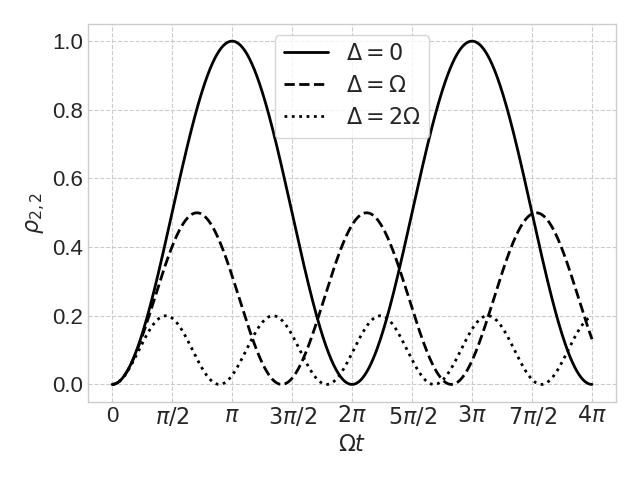
\includegraphics[width=0.5\textwidth]{USPSC-img/Rabi_oscillations.png}
	\legend{Population of the excited state for Rabi oscillations with detunings equal to $ 0 $ (exact resonance), $ \Omega $, and $ 2\Omega $. \\ Source: Author}
	\label{fig:Rabi-oscillations}
	\vspace{-15pt}
\end{figure}

In the exact resonance given by the equations (\ref{eq:population-inversion-exact-resonance-strong-excitation}) and (\ref{eq:coherence-exact-resonance-strong-excitation}), the period is $ T = 2\pi / \Omega $. If a field is turned on at $ t = 0 $ and then turned off after $ t = T / 2 $, an atom initially in the ground state will be certainly promoted to the excited state. Such pulse is called \textbf{$\pi$-pulse}. Furthermore, if a filed is turned on for a duration $ T / 4 $, an atom initially in the ground state ends up in a superposition between the excited and ground states, which is called \textbf{$\pi/2$-pulse}. This is widely used in atomic clocks and quantum computation, beyond the scope of this thesis.

When spontaneous emission is consirable, the Rabi oscillations will be damped by them so that, after a while, the system will reach the steady-state given by (\ref{eq:stationary-population-inversion}) and ({\ref{eq:stationary-coherence}). To get some insight into the damping oscillations, let us analyze the case of exact resonance $ \Delta = 0 $, which has a friendly exact solution. Afterwards, we perform numerical calculations to evaluate the dependence of the damping coefficients $ a $ and $ b $, and the oscillation frequency $ c $ in (\ref{eq:general-solution-OBEs}) with the parameters $ \Omega $, $ \Delta $, and $ \Gamma $.

In the exact resonance case $ \Delta = 0 $, the roots of the characteristic polynomial (\ref{eq:characteristic-polynomial}) have a friendly form given by
\begin{gather}
	m_1 = -\frac{\Gamma}{2},\ \ m_2 = - \left(\frac{3 \Gamma}{4} + i \Omega_{\Gamma} \right),\ \ m_3 = - \left(\frac{3 \Gamma}{4} - i \Omega_{\Gamma} \right),
	\label{eq:eigenvalues-damped-Rabi-oscillations}
\end{gather}
where $ \Omega_{\Gamma} \equiv \sqrt{\Omega^2 - (\Gamma / 4)^2} $ is the Rabi oscillations frequency in the presence of damping. Plugging these eigenvalues in $ \mathcal{M}\vec{\chi}_i = m_i \vec{\chi} $, we obtain the following eigenvectors
\begin{equation}
	 \vec{\chi}_1 = \left[ \begin{matrix} 1 \\ 0 \\ 0 \end{matrix} \right],\ \
	 \vec{\chi}_2 = \left[ \begin{matrix} 0 \\ 1 \\ e^{i\theta} \end{matrix} \right],\ \
	 \vec{\chi}_3 = \left[ \begin{matrix} 0 \\ 1 \\ e^{-i\theta} \end{matrix} \right],
	\label{eq:eigenvectors-damped-Rabi-oscillations}
\end{equation}
where $ \tan \theta = 4 \Omega_{\Gamma} / \Gamma $. Again, let us consider an atom initially in the ground state so that
\begin{equation}
	\vec{\xi}(0) = \mathbf{a}(0) - \mathbf{a}(\infty) = \left[ \begin{matrix} 0 \\ 0 \\ 1 \end{matrix} \right] - \left[ \begin{matrix} 2\Re[q(\infty)] \\ 2\Im[q(\infty)] \\ p(\infty) \end{matrix} \right] = (1 - p(\infty)) \left[ \begin{matrix} 0 \\ \Gamma / \Omega \\ 1 \end{matrix} \right].
	\label{eq:initial-conditions-damped-Rabi-oscillations}
\end{equation}
Thus, plugging the values (\ref{eq:eigenvalues-damped-Rabi-oscillations}) and (\ref{eq:eigenvectors-damped-Rabi-oscillations}) in (\ref{eq:superposition-Bloch-vector-2}) and assuming the initial conditions (\ref{eq:initial-conditions-damped-Rabi-oscillations}), we obtain
\begin{equation}
	c_1 \left[ \begin{matrix} 1 \\ 0 \\ 0 \end{matrix} \right] + c_2 \left[ \begin{matrix} 0 \\ 1 \\ e^{i\theta} \end{matrix} \right] + c_3 \left[ \begin{matrix} 0 \\ 1 \\ e^{-i\theta} \end{matrix} \right] = (1 - p(\infty)) \left[ \begin{matrix} 0 \\ \Gamma / \Omega \\ 1 \end{matrix} \right],
	\label{eq:evaluating-initial-conditions-damped-Rabi-oscillations}
\end{equation}
which is a system of linear equations. After some algebra, the solution of (\ref{eq:evaluating-initial-conditions-damped-Rabi-oscillations}) is
\begin{equation}
	c_1 = 0,\ \ c_2 = c_3^* = \left[ \frac{\Gamma}{2\Omega} - i \frac{\Omega^2 - \Gamma^2 / 4}{2 \Omega \Omega_{\Gamma}} \right](1 - p(\infty)).
	\label{eq:constants-damped-Rabi-oscillations}
\end{equation}
Then, we plug (\ref{eq:constants-damped-Rabi-oscillations}), (\ref{eq:eigenvalues-damped-Rabi-oscillations}), and (\ref{eq:eigenvectors-damped-Rabi-oscillations}) in (\ref{eq:superposition-Bloch-vector-2}), obtaining
\begin{align}
	p_{\xi}(t) &= e^{-3\Gamma t / 4}(1 - p(\infty))\left[\cos(\Omega_{\Gamma}t) + \frac{3\Gamma}{4 \Omega_{\Gamma}} \sin(\Omega_{\Gamma}t) \right]\ \ \textrm{and}
	\label{eq:xi-population-inversion-damped-Rabi-oscilations}
	\\
	q_{\xi}(t) &= ie^{-3\Gamma t / 4} (1 - p(\infty)) \frac{\Gamma}{2\Omega} \left[\cos(\Omega_{\Gamma}t) - \frac{\Omega^2 - \Gamma^2 / 4}{\Gamma \Omega_{\Gamma}} \sin(\Omega_{\Gamma}t) \right].
	\label{eq:xi-coherence-damped-Rabi-oscilations}
\end{align}
Finally, plugging the equations (\ref{eq:xi-population-inversion-damped-Rabi-oscilations}) and (\ref{eq:xi-coherence-damped-Rabi-oscilations}) in $ \mathbf{a}(t) = \vec{\xi}(t) + \mathbf{a}(\infty) $, we obtain
\begin{align}
	p(t) &= e^{-3\Gamma t / 4}(1 - p(\infty))\left[\cos(\Omega_{\Gamma}t) + \frac{3\Gamma}{4 \Omega_{\Gamma}} \sin(\Omega_{\Gamma}t) \right] + p(\infty)\ \ \textrm{and}
	\label{eq:population-inversion-damped-Rabi-oscillations}
	\\
	q(t) &= i(1 - p(\infty)) \frac{\Gamma}{2\Omega} \left\{ e^{-3\Gamma t / 4} \left[\cos(\Omega_{\Gamma}t) - \frac{\Omega^2 - \Gamma^2 / 4}{\Gamma \Omega_{\Gamma}} \sin(\Omega_{\Gamma}t) \right] - 1 \right\}.
	\label{eq:coherence-damped-Rabi-oscillations}
\end{align}
The equation (\ref{eq:population-inversion-damped-Rabi-oscillations}) shows a \textit{damped oscillation} illustrated in figure \ref{fig:damped-Rabi-oscillations}. The damping effect is as strong as the spontaneous emission so that the oscillation vanishes at a decay rate $ 3\Gamma/4 $. Furthermore, when $ \Gamma $ approaches $ 4\Omega $, the oscillations also vanish since $ \Omega_{\Gamma} $ tends to zero.

\begin{figure}[!ht]
	\centering
	\caption{Damped Rabi oscillations}
	\vspace{-10pt}
	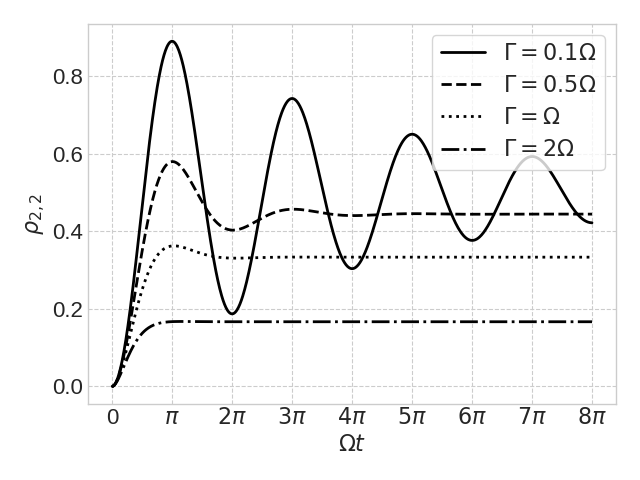
\includegraphics[width=0.5\textwidth]{USPSC-img/Damped_Rabi_oscillations.png}
	\legend{Source: Author \\ Population of the excited state for damped Rabi oscillations with relaxation rates equal to $ 0 $ (exact resonance), $ \Omega/2 $, $ \Omega $, and $ 2\Omega $.}
	\label{fig:damped-Rabi-oscillations}
	\vspace{-15pt}
\end{figure}

There is not a simple analytical solution for the general case (\ref{eq:general-solution-OBEs}) since the roots of the characteristic polynomial (\ref{eq:characteristic-polynomial}) do not have a friendly form out of specific regimes such as strong excitation (section \ref{sec:Rabi-oscillations}) and exact resonance (\ref{sec:exact-resonance}). Then, to evaluate the coefficients $ a $ and $ b $, and the oscillation frequency $ c $, we numerically calculate the eigenvalues of $ \mathcal{M} $. These eigenvalues are associated with the coefficients $ a $, $ b $, and $ c $ through (\ref{eq:general-form-eigenvalues}).

\begin{figure}[H]
	\caption{Damping coefficients $ a $ and $ b $}
	\begin{subfigure}[t]{0.48\textwidth}
		\centering
		\subcaption{Damping coefficient $ a $}
		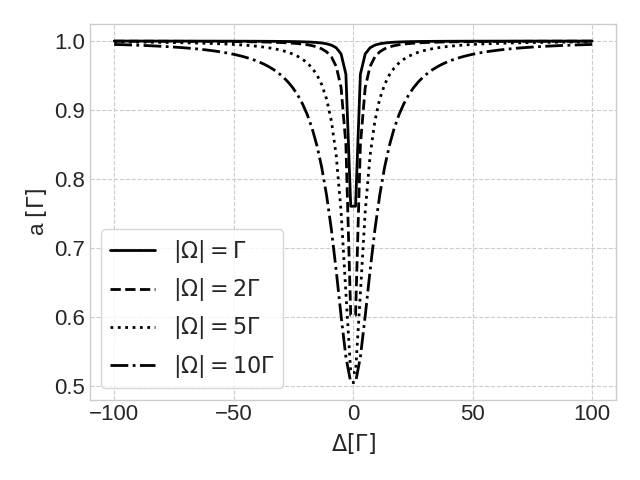
\includegraphics[width=1.0\textwidth]{USPSC-img/damping_coefficient_a.png}
		\vspace{-5pt}
		\legend{Damping coefficient $ a $ from equation (\ref{eq:general-solution-OBEs}) in function of the detuning $ \Delta $ for different Rabi frequencies $ \Omega $.}
	\label{fig:damping-coefficient-a}
	\end{subfigure}
	\hfill
	\begin{subfigure}[t]{0.48\textwidth}
		\centering
		\subcaption{Damping coefficient $ b $}
		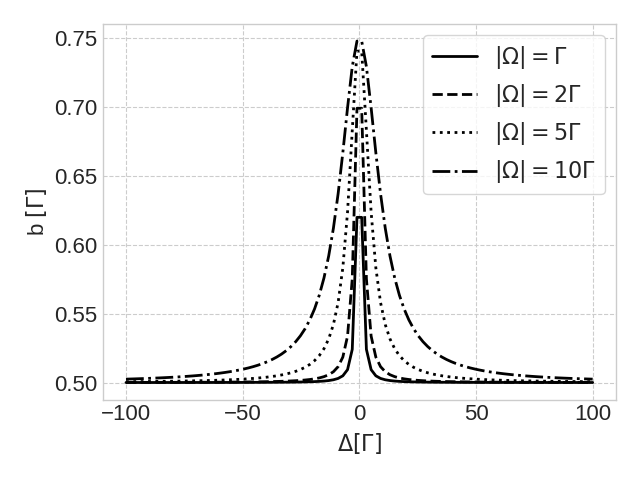
\includegraphics[width=1.0\textwidth]{USPSC-img/damping_coefficient_b.png}
		\vspace{-5pt}
		\legend{Damping coefficient $ b $ from equation (\ref{eq:general-solution-OBEs}) in function of the detuning $ \Delta $ for different Rabi frequencies $ \Omega $.}
		\label{fig:damping-coefficient-b}
	\end{subfigure}

	\legend{Source: Author}
	\label{fig:damping-coefficients}
	\vspace{-30pt}
\end{figure}
The damping coefficient $ a $ from equation (\ref{eq:general-solution-OBEs}) is the rate at which the populations and coherences decay. From figure \ref{fig:damping-coefficient-a}, we can see that $ a $ converges to $ \Gamma $ when $ a \rightarrow \pm \infty $. Also, the coefficient $ a $ is between $ \Gamma/2 $ and $ \Gamma $. The damping coefficient $ b $ from equation (\ref{eq:general-solution-OBEs}) is a rate at which the Rabi oscillations decay. From figure \ref{fig:damping-coefficient-b}, we can see that $ b $ converges to $ \Gamma / 2 $ when $ b \rightarrow \pm \infty $ and it is between $ \Gamma / 2 $ and $ 3\Gamma/4 $. The lower the Rabi frequency the faster $ a $ and $ b $ converge. The system practically reaches the steady-state for a time greater than $ 2 / \Gamma $, since both damping coefficients have the minimum $ \Gamma / 2 $.

\begin{figure}[!ht]
	\centering
	\caption{Oscillation frequency $ c $}
	\vspace{-10pt}
	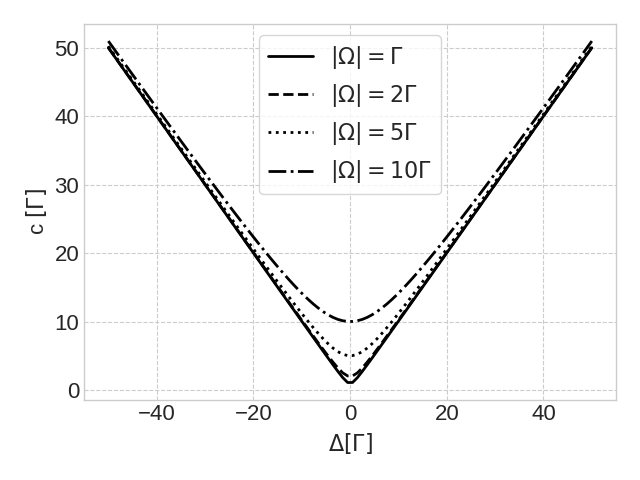
\includegraphics[width=0.5\textwidth]{USPSC-img/oscillation_frequency_c.png}
	\legend{Source: Author \\ Oscillation frequency $ c $ from equation (\ref{eq:general-solution-OBEs}) in function of the detuning $ \Delta $ for different Rabi frequencies $ \Omega $.}
	\label{fig:oscillation-frequency-c}
	\vspace{-15pt}
\end{figure}

The coefficient $ c $ from equation (\ref{eq:general-solution-OBEs}) is the frequency at which the system oscillates (Rabi oscillations). From figure \ref{fig:oscillation-frequency-c}, we can see that $ c $ increases linearly for higher detunings so that $ c = |\Delta| $. For lower detunings, $ c $ converges to $ \Omega_{\Gamma} = \sqrt{\Omega^2 - (\Gamma/4)^2} $.

%-----------------------------------
\subsection{Rate-equation limit}
\label{sec:rate-equation-limit}
%-----------------------------------

The OBEs become the Einstein rate equations when the coherent effects do not play a role. Then, we can derived the Einstein equations eliminating the coherence $ q $ in the OBEs adiabatically. Let us assume a slow population dynamics so that the coherence decay much faster than the populations. Thus, $ \partial_t q \simeq 0 $ in the time scale of the population dynamics. This is called \textbf{adiabatic approximation} and it is valid when there is a considerable collision rate\footnote{The collision rate is associated with pure dephasing terms in the Lindblad superoperator (\ref{eq:Lindblad-superoperator})} $ \gamma $ so that $ \gamma \gg \Gamma, \Omega $. In this regime, from equations (\ref{eq:optical-Bloch-equations-1}), (\ref{eq:optical-Bloch-equations-2}), (\ref{eq:optical-Bloch-equations-3}) and (\ref{eq:optical-Bloch-equations-4}), we obtain
\begin{equation}
	\partial_t \rho_{2,2} = (1 - 2\rho_{2,2})\frac{\Omega}{2}\frac{2\Omega / \Gamma}{1 + (2\Delta / \Gamma)^2} - \Gamma \rho_{2,2},
	\label{eq:population-excited-state-adiabatic-approximation}
\end{equation}
where we assume $ \partial_t \rho_{1,2} = \partial_t \rho_{2,1} = 0 $ and $ \rho_{1,1} = 1 - \rho_{22} $. Comparing equations (\ref{eq:population-excited-state-adiabatic-approximation}) and (\ref{eq:distribution-excited-state-monochromatic-light}), we associate
\begin{equation}
	A \rightarrow \Gamma \ \ \textrm{and}\ \ \alpha(\Delta) = \Omega\frac{2\Omega / \Gamma}{1 + (2\Delta / \Gamma)^2},
\end{equation}
where $ \alpha $ is the \textit{pumping rate}. Therefore, the \textit{saturation parameter} $ s(\Delta) = \alpha(\Delta) / A $ is given by
\begin{equation}
	s(\Delta) = \frac{2\Omega^2 / \Gamma^2}{1 + (2\Delta / \Gamma)^2} = \frac{s_0}{1 + (2\Delta/\Gamma)^2},\ \ s_0 \equiv s(0) = \frac{2\Omega^2}{\Gamma^2},
	\label{eq:saturation-parameter-OBEs}
\end{equation}
where $ s_0 $ is the \textbf{resonant saturation parameter}. Thus, comparing equations (\ref{eq:saturation-parameter-ERE}) and (\ref{eq:saturation-parameter-OBEs}), we obtain
\begin{equation}
	s_0 = \frac{I_0}{I_s} = \frac{2\Omega^2}{\Gamma^2}\ \ \textrm{and}\ \ g(\Delta) = \frac{g(0)}{1 + (2\Delta/\Gamma)^2},
\end{equation}
where $ g(\Delta) $ is the \textit{line shape function} and $ I_s $ is the \textit{saturation parameter}. Since $ g $ must be normalized, we have
\begin{equation}
	\int_{-\infty}^{\infty} g(\Delta) d\Delta = 1 \Rightarrow g(0) = \frac{2}{\pi \Gamma} \Rightarrow g(\Delta) = \frac{1}{\pi} \frac{\Gamma/2}{\Delta^2 + (\Gamma/2)^2} = \frac{2}{\pi \Gamma} \frac{1}{1 + (2\Delta / \Gamma)^2},
	\label{eq:line-shape-function-2}
\end{equation}
where $ g(\Delta) $ is a \textit{Lorentzian function} whose centre is at $ \Delta = 0 $ and FWHM is $ \Gamma $. From equations (\ref{eq:absorption-cross-section-2}), (\ref{eq:net-absorption-cross-section-2}), and (\ref{eq:saturation-parameter-OBEs}), we obtain
\begin{gather}
	\sigma(\Delta) = \frac{\hbar \omega_0}{I_s} \frac{\Gamma}{2} \frac{1}{1 + (2\Delta/\Gamma)^2} = \frac{\sigma_0}{1 + (2\Delta / \Gamma)^2}\ \ \textrm{and}
	\label{eq:absorption-cross-section-3}
	\\
	\sigma_{abs}(\Delta) = \frac{\hbar \omega_0}{I_0} \frac{\Gamma}{2} \frac{s_0}{1 + s_0 + (2\Delta / \Gamma)^2} = \frac{\sigma_0}{1 + s_0 + (2\Delta / \Gamma)^2}.
	\label{eq:net-absorption-cross-section-3}
\end{gather}

Even if $ \partial_t q $ is not negligible, i.e. the coherence and populations dynamics are in the same time scale, it is possible to compare the stationary solution of the OBEs and the Einstein equations in thermal equilibrium. In this case, we should obtain the same equations deduced above if we compare (\ref{eq:probability-excited-state-monochromatic-light}) and (\ref{eq:stationary-excited-state-population}).

It is convenient to rewrite equations (\ref{eq:stationary-population-inversion}) and (\ref{eq:stationary-coherence}) in terms of the saturation parameter so that
\begin{gather}
	p(\infty) = \frac{1}{1 + s(\Delta)} = \frac{1 + (2\Delta / \Gamma)^2}{1 + s_0 + (2\Delta / \Gamma)^2},
	\label{eq:population-inversion-OBEs-2}
	\\
	q(\infty) = \rho_{2,1} = \frac{\Gamma}{2\Omega} \frac{s(\Delta)}{1 + s(\Delta)} (2\Delta / \Gamma - i) = \frac{\Gamma}{2\Omega} \frac{s_0}{1 + s_0 + (2\Delta/\Gamma)^2} (2\Delta / \Gamma - i).
	\label{eq:coherence-OBEs-2}
\end{gather}

%-----------------------------------
\subsection{Line-broadening mechanisms}
\label{sec:line-broadening-mechanisms}
%-----------------------------------

In section \ref{sec:spectral-broadening}, we introduce the \textit{line shape function} $ g(\omega) $, which gives the probability of either absorbing or emitting a photon with a frequency between $ \omega $ and $ \omega + d\omega $. This function is proportional to the \textit{absorption cross-section} $ \sigma(\omega) $ according equation (\ref{eq:absorption-cross-section-2}). Although the line shape function take spectral broadening into account, it is not directly proportional to both absorbing and fluorescence profiles, which are actually measured. Theses profiles are associated directly with the \textit{net absorption cross-section} $ \sigma_{abs} $ and the \textit{scattering cross-section} $ \sigma_{sc} $. From equations (\ref{eq:net-absorption-cross-section-3}) and (\ref{eq:scattering-cross-section}), we can see that the absorption profile is not a sharp line as discussed in section \ref{sec:spectral-broadening}. In the next sections, we shall discuss physical effects which can both broaden and shift the absorption/scattering cross-section profile. Overall, there are two types of line broadening mechanisms:
\begin{itemize}
	\item \textbf{Homogeneous broadening:} all atoms in a medium are affected in the same way. In this case, we can add these line-broadening mechanisms in the optical Bloch equations so that it is valid for all atoms in the medium;

	\item \textbf{Inhomogeneous broadening:} each atom in a medium is individually affected. In this case, we can only described line-broadening mechanisms in the optical Bloch equations for individual atoms. Therefore, we can not generalize for all atoms in the medium.
\end{itemize}

Let us assume an isolated atom initially in the excited state so that there is not an incident light beam ($ s_0 = 0 $). This atom will decay in an average time $ 1/\Gamma $ known as \textit{lifetime}. In other words, $ 1 / \Gamma $ is the average time for the system changes considerably. Therefore, due to the \textit{time-energy uncertainty principle}, there will be an energy uncertainty in the excited state given by
\begin{equation}
	\Delta E \geq \frac{\hbar}{2\Delta t} = \frac{\hbar\Gamma}{2}.
\end{equation}
\begin{figure}[!ht]
	\centering
	\vspace{0pt}
	\caption{Natural broadening}
	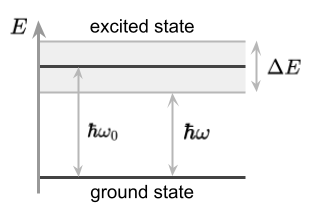
\includegraphics[width=0.4\textwidth]{USPSC-img/natural_broadening.png}
	\vspace{5pt}
	\legend{Energy uncertainty of a excited state whose lifetime is $ 1/\Gamma $. Due to the time-energy uncertainty principle, $ \Delta E \geq \hbar \Gamma / 2 $ and then a spontaneously emitted photon have a random energy $ \hbar \omega $ whose the average is $ \hbar \omega_0 $ and the uncertainty is greater than $ \hbar \Gamma / 2 $.\\ Source: Author}
	\vspace{-10pt}
	\label{fig:natural-broadening}
\end{figure}
Spontaneously emitted photons do not have a deterministic energy $ \hbar \omega_0 $ since the system does not have either, as illustrated in figure \ref{fig:natural-broadening}. This phenomena provokes a \textit{homogeneous} line-broadening known as \textbf{natural broadening} or \textbf{lifetime broadening}. The probability of spontaneously emitting a photon with frequency between $ \omega $ and $ \omega + d\omega $ is given by the line shape function $ g(\omega) $ and it is proportional to the absorption cross-section $ \sigma(\omega) $ according equations (\ref{eq:line-shape-function-2}) and (\ref{eq:absorption-cross-section-3}). From equation (\ref{eq:line-shape-function-2}), we have
\begin{equation}
	g(\Delta) = \frac{1}{\pi} \frac{\Gamma / 2}{\Delta^2 + (\Gamma / 2)^2}.
	\label{eq:line-shape-function-natural-broadening}
\end{equation}
The equation (\ref{eq:line-shape-function-natural-broadening}) is \textit{Lorentzian profile} whose FWHM, also known as \textit{linewidth}, is $ \Gamma $, which is in agreement to equation (\ref{eq:line-shape-simplest-case}) proposed in section \ref{sec:spectral-broadening}. Since $ \Gamma $ is associated with the natural broadening, it is also called \textbf{natural linewidth}. In the regime of weak excitation so that $ s_0 \ll 1 $, the absorption cross-section approximately equals the net absorption cross-section such that $ \sigma \simeq \sigma_{abs} $.

In the presence of a light field so that $ s_0 > 0 $, the only spectral broadening is the natural broadening given by (\ref{eq:line-shape-function-natural-broadening}). However, the net absorption cross-section $ \sigma_{abs} $ does not equal the absorption cross-section $ \sigma $. According to equation (\ref{eq:net-absorption-cross-section-2}), there will be a decreasing by a factor of $ 1 + s(\omega) $, which causes a line-broadening illustrated in figure (\ref{fig:net-absorption-cross-section}). From equations (\ref{eq:net-absorption-cross-section-3}) and (\ref{eq:absorption-cross-section-3}), we have
\begin{gather}
	\sigma(\Delta) = \frac{\pi \Gamma \sigma_0}{2} g(\Delta)\ \ \textrm{and}\ \ \sigma_{abs}(\Delta) = \frac{\pi \Gamma \sigma_0}{2(1 + s_0)} L(\Delta),
	\\
	\textrm{where}\ \ L(\Delta) \equiv \frac{2}{\pi \Gamma'} \frac{1}{1 + (2\Delta / \Gamma')^2}\ \ \textrm{and}\ \ \Gamma' \equiv \Gamma \sqrt{1 + s_0}.
	\label{eq:absorption-line-shape}
\end{gather}
The function $ L $ is known as \textbf{absorption line-shape} and it is a \textit{Lorentzian profile} whose \textit{FWHM} is $ \Gamma' $. The quantity $ \Gamma' $ is known as \textbf{power-broadened linewidth}. In the regime of weak excitation so that $ s_0 \ll 1 $, the absorption line-shape becomes the line shape function, $ L(\Delta) \rightarrow g(\Delta) $, and the power-broadened linewidth becomes the natural linewidth, $ \Gamma' \rightarrow \Gamma $.

\begin{figure}[!ht]
	\centering
	\caption{Net absorption cross-section}
	\vspace{-5pt}
	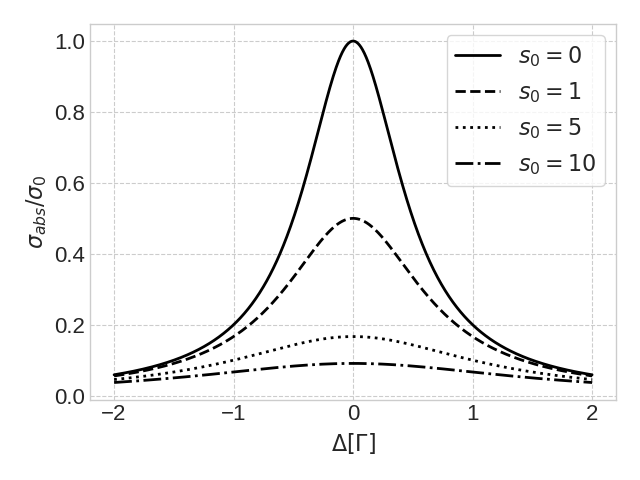
\includegraphics[width=0.5\textwidth]{USPSC-img/net_absorption_cross_section.png}
	\vspace{-5pt}
	\legend{Net absorption cross section as function of detuning for some values of resonant saturation parameter.\\ Source: Author}
	\label{fig:net-absorption-cross-section}
\end{figure}

The angular frequency $ \omega' $ of an incident light beam depends on the frame in which it is being observed. This effect is known as \textbf{Doppler effect}. We have been studying the atom-light interaction assuming that the light frequency is the same in both laboratory and atom frames. However, the Doppler effect causes an \textit{inhomogeneous resonance shift} since each atom will perceive an angular frequency given by
\begin{equation}
	\omega' = \omega - \mathbf{k} \cdot \mathbf{v},
	\label{eq:Doppler-effect}
\end{equation}
where $ \omega $ and $ \mathbf{k} $ are, respectively, the angular frequency and the wave vector of the light beam in the laboratory frame, and $ \mathbf{v} $ is the velocity of the atom also in the laboratory frame. Subtracting the resonant angular frequency $ \omega_0 $ in both sides of equation (\ref{eq:Doppler-effect}), we obtain
\begin{equation}
	\Delta_{eff} = \Delta - \mathbf{k} \cdot \mathbf{v},
	\label{eq:Doppler-shift}
\end{equation}
where $ \Delta_{eff} = \omega' - \omega_0 $ is the \textit{effective detuning}. We must called $ -\mathbf{k} \cdot \mathbf{v} $ as \textbf{Doppler shift}. Let us consider a gas following the \textit{Maxwell-Boltzmann distribution} so that the probability $ P(v) dv $ of finding an atom with a velocity component between $ v $ and $ v + dv $ parallel to $ \mathbf{k} $ direction is given by
\begin{equation}
	P(v) dv = \frac{1}{\alpha\sqrt{2\pi}} \exp\left(-\frac{v^2}{2\alpha^2}\right) dv,\ \ \alpha \equiv \sqrt{\frac{k_B T}{m}},
	\label{eq:Maxwell-Boltzmann-distribution}
\end{equation}
where $ T $ is the temperature of the gas, $ k_B $ is the Boltzmann constant, and $ m $ is the atom mass. The equation (\ref{eq:Maxwell-Boltzmann-distribution}) is a \textbf{Gaussian distribution} centered at zero whose \textit{standard deviation} is $ \alpha $. Also, the FWHM is approximately $ 2.355 \alpha $. If we consider a resonant laser so that $ \Delta = 0 $ or $ \omega = \omega_0 $, we can associated an effective absorption line shape given by
\begin{equation}
	D(\omega') = \frac{1}{\beta \sqrt{2\pi}} \exp\left[-\frac{(\omega' - \omega_0)^2}{2\beta^2}\right],\ \ \beta \equiv \frac{\omega_0}{c} \alpha = \frac{\omega_0}{c} \sqrt{\frac{k_b T}{m}}.
\end{equation}

%-----------------------------------
\subsection{Optical forces}
\label{sec:optical-forces}
%-----------------------------------

We can divide the atom state into two sets. The first one is the \textit{internal states} related to the \textit{electronic states}. The second one is the \textit{external states} associated with the centre-of-mass coordinates. So far we evaluated the dynamics of the internal states, neglecting the dynamics of the atomic centre-of-mass except to explain Doppler broadening in section (\ref{sec:line-broadening-mechanisms}). However, there is a coupling between the external and internal degrees of freedom mediated by the absorption and emission processes, which provokes mechanical effects in the atomic centre-of-mass. These effects can be quantify from the \textit{Ehrenfest theorem}, which establishes the average force given by
\begin{equation}
	\mathbf{F} = - \braket{\nabla \hat{V}},
	\label{eq:average-force}
\end{equation}
where $ \hat{V} $ is the interaction Hamiltonian.

In section \ref{sec:interaction-Hamiltonian}, we introduce the interaction Hamiltonian assuming an interaction between a two-level atom and a monochromatic light beam in the \textit{rotating frame} and in the \textit{interaction picture}. In the dynamics of the internal states, we can neglect the spatial dependence of the Rabi frequency $ \Omega $ due to the rotating wave approximation. However, in the dynamics of the external states this spatial variation must be considered. It is important to notice that $ E_0 $ can have a spatial dependence by itself when the light beam is not a plane wave, which is the case of a Gaussian beam\footnote{The Gaussian beam properly described that light beam produces by a laser.}. Considering $ \Omega(\mathbf{r}) = |\Omega(\mathbf{r})| e^{i\mathbf{k}\cdot\mathbf{r}} $\footnote{Any additional phase in $ \Omega $ can be incorporated in the coherence $ q $}, we obtain
\begin{align}
	\hat{V}(\mathbf{r}) &= \frac{\hbar}{2}\left[ \begin{matrix} 0 & |\Omega(\mathbf{r})| e^{-i\mathbf{k}\cdot\mathbf{r}} \\ |\Omega(\mathbf{r})| e^{i\mathbf{k}\cdot\mathbf{r}} & -2\Delta \end{matrix} \right] \Rightarrow \\
	\nabla \hat{V} &= \frac{\hbar}{2}\left[ \begin{matrix} 0 & (\nabla|\Omega| - i\mathbf{k}|\Omega|)e^{-i\mathbf{k}\cdot\mathbf{r}} \\ (\nabla|\Omega| + i\mathbf{k}|\Omega|) e^{i\mathbf{k}\cdot\mathbf{r}} & 0 \end{matrix} \right],
\end{align}
We can evaluate the average force (\ref{eq:average-force}) considering the property (\ref{eq:trace-average}) so that
\begin{equation}
	\mathbf{F} = -\Tr[\hat{\rho}\nabla\hat{V}],
\end{equation}
where $ \hat{\rho} $ is the density operator of the two-level atom. As discussed in section \ref{sec:optical-Bloch-equations}, the system will reach a steady-state due to spontaneous emission, a relaxation process. We also verify that the system reaches the steady-state exponentially at a minimum rate $ \Gamma / 2 $, where $ \Gamma $ is the natural linewidth. If the dynamics time scale is much greater than $ 2 / \Gamma $, we can assume the system in the steady-state. Then, the density operator $ \hat{\rho} $ are defined by equations (\ref{eq:stationary-population-inversion}) and (\ref{eq:stationary-coherence}) and the average force $ \mathbf{F} $ is given by
\begin{equation}
	\mathbf{F} = -\hbar \Re[(\nabla|\Omega| + i\mathbf{k}|\Omega|)q^*(\infty)].
	\label{eq:optical-forces-1}
\end{equation}
Plugging $ q(\infty) $ of equation (\ref{eq:coherence-OBEs-2}) in (\ref{eq:optical-forces-1}), we obtain
\begin{equation}
	\mathbf{F} = -\frac{\hbar \Delta}{\Omega} \frac{s(\Delta)}{1 + s(\Delta)}\nabla \Omega  + \hbar\mathbf{k} \frac{\Gamma}{2} \frac{s(\Delta)}{1 + s(\Delta)}.
	\label{eq:optical-forces-2}
\end{equation}
We can simply the equation (\ref{eq:optical-forces-2}) considering
\begin{equation}
	\nabla \ln\left[1 + s(\Delta) \right] = \frac{2}{\Omega} \frac{s(\Delta)}{1 + s(\Delta)} \nabla \Omega.
	\label{eq:simplification-1}
\end{equation}
Then, plugging (\ref{eq:simplification-1}) in (\ref{eq:optical-forces-2}), we obtain $ \mathbf{F} = \mathbf{F}_{rp} + \mathbf{F}_{dp} $ where
\begin{align}
	\mathbf{F}_{rp} &= \hbar \mathbf{k} \frac{\Gamma}{2} \frac{s(\Delta)}{1 + s(\Delta)} = \hbar \mathbf{k} \frac{\Gamma}{2} \frac{s_0}{1 + s_0 + (2\Delta/\Gamma)^2},
	\label{eq:radiation-pressure-force}
	\\
	\mathbf{F}_{dp} &= -\nabla U_{dp},\ \ U_{dp} = \frac{\hbar \Delta}{2} \ln\left[1 + s(\Delta) \right] = \frac{\hbar \Delta}{2} \ln\left[1 + \frac{s_0}{1 + (2\Delta/\Gamma)^2} \right],
	\label{eq:gradient-dipole-force}
\end{align}
The dissipative force $ \mathbf{F}_{rp} $ is called \textbf{radiation pressure force} and the conservative force $ \mathbf{F}_{dp} $ is called \textbf{gradient dipole force}.

We can rewrite $ \mathbf{F}_{rp} $ from equation (\ref{eq:radiation-pressure-force}) considering the scattering cross-section $ \sigma_{sc} $ from equation (\ref{eq:scattering-cross-section}) so that
\begin{equation}
	\mathbf{F}_{rp} = \hbar \mathbf{k} \frac{I_0}{\hbar \omega_0} \sigma_{sc}(\Delta) = \hbar \mathbf{k} R_{sc},\ \ R_{sc} = \frac{\Gamma}{2}\frac{s_0}{1 + s_0 +  (2\Delta / \Gamma)^2},
	\label{eq:radiation-pressure-force-2}
\end{equation}
where $ I_0 / (\hbar \omega_0) $ is the flux of photons from the incident beam. The quantity $ R_{sc} $, known as \textbf{scattering rate}, is the frequency at which an atom absorbs photons from the incident beam and afterwards scatters them out by spontaneous emission. Hence, from equation (\ref{eq:radiation-pressure-force-2}), we can interpret the radiation pressure force as the gained momentum after successive events of absorption followed by spontaneous emission. Since the spontaneous emission is isotropic, only the absorption events contribute for the gained momentum as shown in figure (\ref{fig:radiation-pressure-force}).

\begin{figure}[!ht]
	\centering
	\caption{Radiation pressure force}
	\vspace{-10pt}
	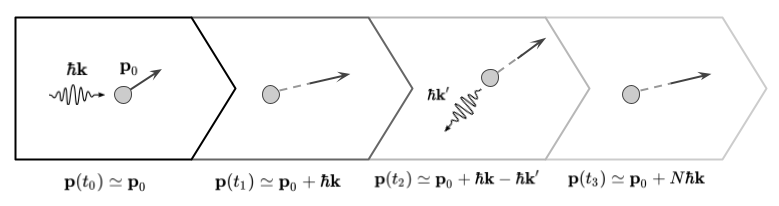
\includegraphics[width=0.8\textwidth]{USPSC-img/radiation_pressure_force.png}
	\vspace{5pt}
	\legend{An atom initially with momentum $ \mathbf{p}_0 $ absorbs a photon with momentum $ \hbar \mathbf{k} $ after a period $ t_1 - t_0 $. Then, at instant $ t_2 $, this atom spontaneously emits a photon with momentum $ \hbar \mathbf{k}' $ so that $ |\mathbf{k}| = |\mathbf{k}'| $. Finally, after successive absorption and emissions, the final momentum will be $ \mathbf{p} \simeq \mathbf{p}_0 + N\hbar\mathbf{k} $ since the spontaneous emission is isotropic. The quantity $ N $ is the number of absorbed photons after a period $ t_3 - t_0 $. Therefore, the impulse after a period $ \Delta t $ will be $ \Delta \mathbf{p} = \hbar \mathbf{k} R_{sc} \Delta t $, where $ R_{sc} $ is the rate at which the atom scatters photons. \\ Source: Author}
	\label{fig:radiation-pressure-force}
	\vspace{-15pt}
\end{figure}

From equation (\ref{eq:radiation-pressure-force-2}), we can see that the radiation pressure force has the maximum at resonance, and it decreases with the detuning. Also, this force saturates when $ s_0 $ is much greater than $ 1 + (2\Delta / \Gamma)^2 $. The spontaneous emission rate determines the force intensity, which is as greater as $ \Gamma $. Since $ \mathbf{F}_{rp} $ is a dissipative force, it can be used to both cool and trap atoms, being a the key concepts to understand MOTs.

The gradient dipole force can be derived from a potential $ U_{dp} $ illustrated in figure (\ref{fig:gradient-dipole-potential}), and therefore it is a conservative force. At resonance, $ U_{dp} $ is zero and its module increases with the detuning for a range near to resonance. Far from resonance, $ U_{dp} $ asymptotically goes into zero. Unlike the radiation pressure force, the gradient dipole force does not saturate. It can increase continuously without bound, though it only does logarithmically for large intensities (saturation parameter). This forces is usually applied to spatially confine atoms.

\begin{figure}[!ht]
	\centering
	\caption{Potential from gradient dipole force}
	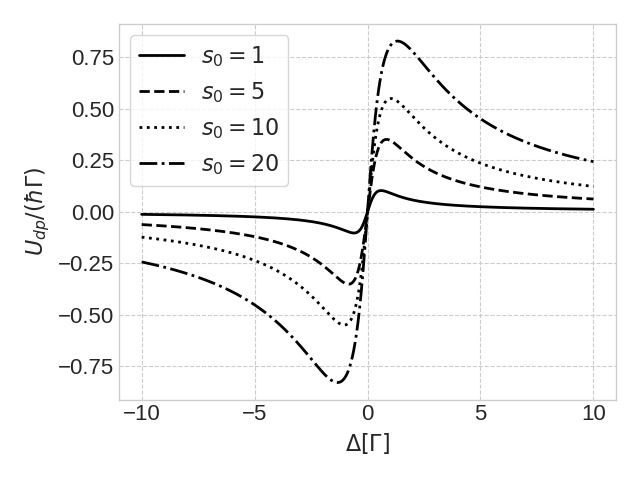
\includegraphics[width=0.5\textwidth]{USPSC-img/gradient_dipole_potential.png}
	\legend{Potential from gradient dipole force for few saturation parameters as a funtion of detuning. \\ Source: Author}
	\label{fig:gradient-dipole-potential}
\end{figure}


%-----------------------------------
